% Options for packages loaded elsewhere
\PassOptionsToPackage{unicode}{hyperref}
\PassOptionsToPackage{hyphens}{url}
%
\documentclass[
  oneside]{scrbook}
\usepackage{amsmath,amssymb}
\usepackage{lmodern}
\usepackage{iftex}
\ifPDFTeX
  \usepackage[T1]{fontenc}
  \usepackage[utf8]{inputenc}
  \usepackage{textcomp} % provide euro and other symbols
\else % if luatex or xetex
  \usepackage{unicode-math}
  \defaultfontfeatures{Scale=MatchLowercase}
  \defaultfontfeatures[\rmfamily]{Ligatures=TeX,Scale=1}
\fi
% Use upquote if available, for straight quotes in verbatim environments
\IfFileExists{upquote.sty}{\usepackage{upquote}}{}
\IfFileExists{microtype.sty}{% use microtype if available
  \usepackage[]{microtype}
  \UseMicrotypeSet[protrusion]{basicmath} % disable protrusion for tt fonts
}{}
\makeatletter
\@ifundefined{KOMAClassName}{% if non-KOMA class
  \IfFileExists{parskip.sty}{%
    \usepackage{parskip}
  }{% else
    \setlength{\parindent}{0pt}
    \setlength{\parskip}{6pt plus 2pt minus 1pt}}
}{% if KOMA class
  \KOMAoptions{parskip=half}}
\makeatother
\usepackage{xcolor}
\IfFileExists{xurl.sty}{\usepackage{xurl}}{} % add URL line breaks if available
\IfFileExists{bookmark.sty}{\usepackage{bookmark}}{\usepackage{hyperref}}
\hypersetup{
  pdftitle={Relatório de rotas e áreas de concentração de aves migratórias no Brasil},
  pdfauthor={Centro Nacional de Pesquisa e Conservação de Aves Silvestres - CEMAVE},
  hidelinks,
  pdfcreator={LaTeX via pandoc}}
\urlstyle{same} % disable monospaced font for URLs
\usepackage{longtable,booktabs,array}
\usepackage{calc} % for calculating minipage widths
% Correct order of tables after \paragraph or \subparagraph
\usepackage{etoolbox}
\makeatletter
\patchcmd\longtable{\par}{\if@noskipsec\mbox{}\fi\par}{}{}
\makeatother
% Allow footnotes in longtable head/foot
\IfFileExists{footnotehyper.sty}{\usepackage{footnotehyper}}{\usepackage{footnote}}
\makesavenoteenv{longtable}
% Make links footnotes instead of hotlinks:
\DeclareRobustCommand{\href}[2]{#2\footnote{\url{#1}}}
\setlength{\emergencystretch}{3em} % prevent overfull lines
\providecommand{\tightlist}{%
  \setlength{\itemsep}{0pt}\setlength{\parskip}{0pt}}
\setcounter{secnumdepth}{5}
\usepackage{booktabs}
\usepackage{pdfpages}
\usepackage[portuguese]{babel}
\selectlanguage{portuguese}
\usepackage{booktabs}
\usepackage{longtable}
\usepackage{array}
\usepackage{multirow}
\usepackage{wrapfig}
\usepackage{float}
\usepackage{colortbl}
\usepackage{pdflscape}
\usepackage{tabu}
\usepackage{threeparttable}
\usepackage{threeparttablex}
\usepackage[normalem]{ulem}
\usepackage{makecell}
\usepackage{xcolor}
\ifLuaTeX
  \usepackage{selnolig}  % disable illegal ligatures
\fi
\usepackage[]{natbib}
\bibliographystyle{apalike}

\title{Relatório de rotas e áreas de concentração de aves migratórias no Brasil}
\author{Centro Nacional de Pesquisa e Conservação de Aves Silvestres - CEMAVE}
\date{}

%\begin{document}
%%%%\maketitle
%%%
\begin{document}
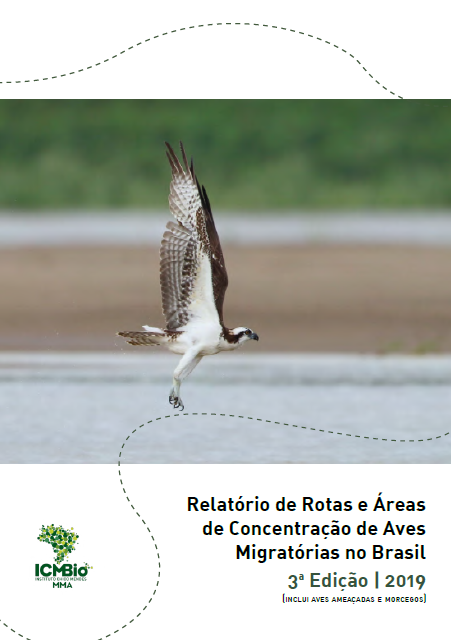
\includepdf{imagens/capa.png}
\maketitle

{
\setcounter{tocdepth}{1}
\tableofcontents
}
\pagestyle{plain}

\hypertarget{apresentacao}{%
\chapter*{Apresentação}\label{apresentacao}}
\addcontentsline{toc}{chapter}{Apresentação}

O Brasil é um país megadiverso que abriga mais de 13\% da riqueza de espécies do globo. É o terceiro país em número de espécies de aves. Das 1.919 espécies atualmente registradas pelo Comitê Brasileiro de Registros Ornitológicos, pouco mais de 10\% são atualmente definidas como migratórias, mas este número ainda pode aumentar conforme cresça o conhecimento sobre o grupo.

Ao longo de sua rota migratória, as aves utilizam diversas áreas para descanso e alimentação. Sem essas áreas, as aves não são capazes de atingir o destino final, deixando de completar seu ciclo de vida. Algumas espécies migratórias têm suas rotas restritas ao território nacional; outras deslocam-se por diversos países vizinhos; outras possuem uma área de distribuição que pode se estender de polo a polo. Essa interconexão notável entre ambientes, biomas, países, continentes e hemisférios executada pelas espécies migratórias torna o Brasil co-responsável frente ao compromisso de conservação da biodiversidade.

Como esperado, o Brasil é signatário de acordos internacionais relacionados à proteção de espécies migratórias e dos habitats por elas utilizados, como a Convenção internacional para Conservação da Fauna, Flora e Belezas Cênicas das Américas (Convenção de Washington), que trata de espécies migratórias em um dos seus capítulos; a Convenção de Ramsar, relativa à conservação de ambientes aquáticos; a Rede Hemisférica de Reservas para Aves Limícolas (aves que buscam alimento nas zonas entre marés, em ambientes alagados ou em áreas marginais a corpos d'água); o Acordo Internacional para a Conservação de Albatrozes e Petréis -- ACAP; o Memorando de Entendimento para a Conservação de Espécies de Aves Migratórias dos Campos Naturais da América do Sul e de seus habitats; a Convenção de Bonn ou Convenção sobre a Conservação das Espécies Migratórias de Animais Silvestres (CMS).

Apesar de todos esses instrumentos voltados para a conservação das espécies migratórias, há uma redução drástica e muitas vezes irreversível de suas áreas críticas de alimentação, reprodução e descanso. Mesmo quando a área crítica não é perdida por completo, ela pode vir a sofrer tal degradação ambiental que seu uso pelas espécies migratórias mais sensíveis se torna inviável. Neste sentido, é importante reconhecer estas áreas críticas e envidar esforços para o uso sustentável desses espaços e seus recursos.

A implatação de parques eólicos têm contribuído cada vez mais para a formação de uma matriz energética brasileira mais limpa e renovável. A geração de energia a partir dos ventos é considerada de baixo impacto ao meio ambiente, mas pode representar uma ameaça a grupos específicos como aves e morcegos. Nessa perspectiva, o Conselho Nacional de Meio Ambiente (CONAMA) publicou a Resolução n° 462, de 24 de julho de 2014, estabelecendo os procedimentos para o licenciamento ambiental de empreendimentos de geração de energia elétrica a partir de fonte eólica em superfície terrestre (onshore), no território brasileiro. Essa resolução prevê que o órgão licenciador deve exigir estudos e relatório de impacto ambiental e realizar audiências públicas quando o empreendimento estiver localizado em áreas de concentração ou rota de aves migratórias, aqui chamadas de Áreas Importantes para Aves, cabendo ao ICMBio/CEMAVE indicá-las, em território nacional, por meio de um relatório, sendo essa sua terceira edição.

A sua elaboração, a exemplo das edições anteriores, foi baseada nos dados e informações disponíveis na literatura científica, em bancos de dados abertos, no processo de avaliação do estado de conservação da avifauna brasileira, nos Planos de Ação Nacionais e nos registros de anilhamento do Sistema Nacional de Anilhamento de Aves Silvestres (SNA). Contudo, o modo de priorização espacial foi aprimorado: houve redução da malha da grade de análise e uso de um software de priorização espacial, que permite considerar a riqueza de cada local e a raridade e vulnerabilidade de cada espécie.

Com o intuito de minimizar potenciais impactos negativos, também são apresentadas recomendações de medidas preventivas ou operacionais já testadas em outros países. Da mesma forma que os relatórios anteriores, este também apresenta o mapa de registros de espécies de aves ameaçadas de extinção, que poderá ser utilizado como referência pelos órgãos licenciadores.

De forma inédita e suplementar, esta publicação também traz informações sobre a fauna de morcegos no Brasil e o risco de colisão modelado deste grupo com estruturas associadas a empreendimentos eólicos. Tal contribuição foi possível graças a boa vontade de pesquisadores da Universidade Federal de Pernambuco e busca levar aos empreendedores e aos órgãos licenciadores a melhor informação sobre o impacto de empreendimentos eólicos nesse grupo tão essencial para os processos ecossistêmicos.

Esse documento alinha-se ao modelo de desenvolvimento responsável, sinalizando a necessidade e a possibilidade de se permitir o crescimento econômico e social sem negligenciar a conservação da biodiversidade.

Está publicaçao está submetida ao seguinte tipo de licença: \href{https://creativecommons.org/licenses/by-nc-nd/4.0/legalcode}{Attribution-NonCommercial-NoDerivatives 4.0 International}.

\hypertarget{creditos}{%
\chapter*{Créditos}\label{creditos}}
\addcontentsline{toc}{chapter}{Créditos}

\textbf{REPÚBLICA FEDERATIVA DO BRASIL}

\emph{Presidente}\\
JAIR MESSIAS BOLSONARO

\emph{Vice-Presidente}\\
ANTÔNIO HAMILTON MARTINS MOURÃO

\textbf{MINISTÉRIO DO MEIO AMBIENTE}

\emph{Ministro}\\
RICARDO DE AQUINO SALLES

\emph{Secretário de Biodiversidade e Floresta}\\
EDUARDO SERRA NEGRA CAMERINI

\textbf{INSTITUTO CHICO MENDES DE CONSERVAÇÃO DA BIODIVERSIDADE}

\emph{Presidente}\\
HOMERO DE GIORGE CERQUEIRA

\emph{Diretor de Pesquisa, Avaliação e Monitoramento da Biodiversidade}\\
MARCOS AURÉLIO VENÂNCIO

\emph{Coordenadora do Centro Nacional de Pesquisa e Conservação de Aves Silvestres}\\
PRISCILLA PRUDENTE DO AMARAL

Diretoria de Pesquisa, Avaliação e Monitoramento da Biodiversidade\\
Coordenação Geral de Estratégias para a Conservação EQSW 103/104 - Centro Administrativo Setor Sudoeste - Bloco D - 1º andar CEP 70670-350 - Brasília/DF - Tel: 61 3341-9055 - Fax: 61 3341-9068\\
www.icmbio.gov.br

\emph{Relatório de Rotas e Áreas de Concentração de Aves Migratórias no Brasil}\\
\emph{3a Edição \textbar{} 2019}

\begin{center}\rule{0.5\linewidth}{0.5pt}\end{center}

\textbf{Documento elaborado por (em ordem alfabética):}

Camila Garcia Gomes\\
Camile Lugarini\\
Danielle Paludo\\
Diego Mendes\\
Manuella Andrade de Souza\\
Marcos de Souza Fialho\\
Mauricio Cavalcante dos Santos\\
Nathalia Alves\\
Patrícia Pereira Serafini\\
Priscilla Prudente do Amaral

\textbf{REVISÃO TÉCNICA}\\
Camila Garcia Gomes\\
Manuella Andrade de Souza\\
Marcos de Souza Fialho\\
Mauricio Cavalcante dos Santos\\
Priscilla Prudente do Amaral

\textbf{MAPAS}\\
Mauricio Cavalcante dos Santos

\textbf{SUPERVISÃO TÉCNICA E REVISÃO FINAL}\\
Marcos de Souza Fialho\\
Mauricio Cavalcante dos Santos\\
Priscilla Prudente do Amaral

\textbf{CAPA, PROJETO GRÁFICO E DIAGRAMAÇÃO}\\
Marília Ferreira

FOTO DA CAPA\\
José Anselmo D'Affonsêca Neto (\emph{Pandion haliaetus})

\textbf{Catalogação na fonte:}\\
Biblioteca do ICMBio

\begin{center}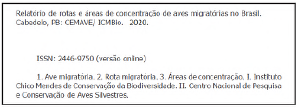
\includegraphics[width=0.75\linewidth]{imagens/ficha} \end{center}

\hypertarget{lista-siglas}{%
\chapter*{Lista de siglas}\label{lista-siglas}}
\addcontentsline{toc}{chapter}{Lista de siglas}

ACAP - Acordo Internacional para a Conservação de Albatrozes e Petréis\\
ANEEL - Agência Nacional de Energia Elétrica APA - Área de Proteção Ambiental\\
APP - Área de Preservação Permanente\\
CBRO - Comitê Brasileiro de Registros Ornitológicos\\
CONAMA - Conselho Nacional de Meio Ambiente\\
CEMAVE - Centro Nacional de Pesquisa e Conservação de Aves Silvestres\\
CMS - Convenção sobre Espécies Migratórias de Animais Selvagens (Convention on Migratory Species)\\
EIA - Estudo de Impacto Ambiental\\
ESEC - Estação Ecológica\\
FLONA - Floresta Nacional\\
IBAMA - Instituto Brasileiro do Meio Ambiente e dos Recursos Naturais Renováveis\\
IBA - Área Importante para Aves (Important Bird Area)\\
ICMBio - Instituto Chico Mendes de Conservação da Biodiversidade\\
MMA - Ministério do Meio Ambiente\\
NDVI - Índice de Vegetação Normalizado\\
PAN - Plano de Ação Nacional\\
REBIO - Reserva Biológica\\
RESEX - Reserva Extrativista\\
RPPN - Reserva Particular do Patrimônio Natural\\
SNA - Sistema Nacional de Anilhamento de Aves Silvestres\\
UNESCO - Organização das Nações Unidas para a Educação, a Ciência e a Cultura

\hypertarget{aves}{%
\chapter{Relatório de rotas e áreas de concentração de aves migratórias no brasil}\label{aves}}

\pagestyle{headings}

\hypertarget{resumo}{%
\section*{Resumo}\label{resumo}}
\addcontentsline{toc}{section}{Resumo}

\emph{Parques eólicos para produção de energia elétrica têm contribuído para a construção de uma matriz energética mais limpa e renovável. No entanto, podem representar uma ameaça a grupos específicos como aves e morcegos. Nessa perspectiva, o Conselho Nacional de Meio Ambiente (CONAMA) publicou uma resolução que prevê que o órgão licenciador deve exigir estudos e relatório de impacto ambiental e realizar audiências públicas quando o empreendimento estiver localizado em áreas de concentração ou rota de aves migratórias, aqui chamadas de Áreas Importantes, cabendo ao ICMBio/CEMAVE indicá-las através do presente relatório, sendo essa sua terceira edição. Para identificar essas Áreas Importantes, realizamos um planejamento sistemático de priorização de áreas ocupadas por espécies sensíveis a empreendimentos eólicos por meio do software Zonation. Somamos a esse resultado áreas de descanso, alimentação ou reprodução que concentram indivíduos de espécies migratórias citadas em publicações científicas ou sugeridas por especialistas. Para o Zonation, estabeleceu-se uma meta de priorização de mais de 90\% das células com registro de ocorrência de espécies migratórias ameaçadas e de 100\% para as raras, ao mesmo tempo em que seleciona as células de maior riqueza de espécies. Das 6.823 células que apresentaram ao menos um registro de espécie migratória, foram priorizadas 2.047 células, ou seja, 30\% das células foram mantidas na solução final. Somando-se a isso, foram apontadas 75 áreas (2.305 células) em 21 estados. Cada área elencada foi identificada, sendo apresentada a justificativa de inclusão e a fonte da informação. Devido a uma disponibilidade desigual de informações, a maior parte das áreas levantadas apresenta ocorrências de espécies migratórias limícolas e costeiro-oceânicas, sendo poucas as áreas regulares de rota, pousio, descanso, alimentação e reprodução para um número expressivo de espécies florestais ou campestres. A área total, considerando as Áreas Importantes por expressiva concentração de indivíduos e as elencadas pelo Zonation, somou 346.262,24 km2 (4.091 células), ou aproximadamente 4\% da superfície do Brasil. Embora todos os estados brasileiros tenham apresentado áreas priorizadas, o padrão geral de distribuição espacial das Áreas Importantes ainda se mostra bastante pulverizado, o que reflete, a despeito do grande número de registros compilados, um cenário com muitas lacunas de conhecimento. Em outras palavras, há muitas áreas com pouco ou nenhum esforço amostral, em especial para a Amazônia e nas áreas distantes de rodovias.}

\hypertarget{abstract}{%
\section*{Abstract}\label{abstract}}
\addcontentsline{toc}{section}{Abstract}

\emph{The energy produced by wind farms has contributed to the creation of a cleaner and renewable energy matrix. However, they can represent a threat to some specific groups such as birds and bats. In this regard, Brazil's National Environment Council (CONAMA) issued a Resolution foreseeing that licensing bodies must demand environmental impact assessments and reports in addition to public hearings whenever an enterprise is located within migratory bird routes or areas of concentration, hereinafter referred as ``Important Areas'', and being ICMBio/CEMAVE charged with the task of indicating these via this report, this being its third edition. To identify these Important Areas, we carried out a systematic priority planning of the areas occupied by wind farm sensitive species using the software Zonation. We added to this result resting, foraging or breeding areas that concentrated individuals of migratory species cited by scientific publications or suggested by experts. For Zonation, a target of prioritizing more than 90\% of cells with an occurrence record of threatened migratory species and 100\% for rare species was set, while selecting cells with the highest species richness. Of the 6,823 cells that presented at least one migratory species record, 2,047 cells were prioritized, that is, 30\% of cells were maintained in the final solutation. Moreover, 75 areas (2,305 cells) were highlighted in 21 states. Each listed area was identified, and the justification for inclusion and information source were presented. Due to an unequal availability in data, most of the areas surveyed present occurrences of shore or coastal-oceanic migratory species, with few regular areas for route, resting, foraging and breeding used by a significant number of forest and grassland species. The total area, considering the Important Areas with significant concentrations of individuals and those Zonation highlighted, totaled 346,262.24 km2 (4,091 cells), or approximately 4\% of Brazil´s surface area. Although all Brazilian states have priority areas, the overall pattern of spatial distribution of the Important Areas still remains quite scattered, which reflects, despite the large number of compiled records, a scenario of many knowledge gaps, in other words, many areas with little or no sampling effort, especially for the Amazon and areas distant from roadways.}

\hypertarget{contextualizacao}{%
\section{Contextualização - Migrações de aves no Brasil}\label{contextualizacao}}

\hypertarget{aves-migratorias}{%
\subsection{Aves Migratórias}\label{aves-migratorias}}

A migração é uma resposta das populações silvestres a uma condição sazonal de baixa disponibilidade de recurso para outra onde o recurso é farto. Para a maioria dos casos, o recurso envolvido é alimento ou área para nidificação (Cornell University 2014), mas a migração também pode estar relacionada à disponibilidade de água ou à diminuição de competição (Able 1999).

Recentemente, Somenzari e colaboradores (2018) revisaram as ocorrências e padrões de deslocamento de aves potencialmente migratórias para o Brasil. Uma espécie foi classificada como migratória quando pelo menos parte de sua população realiza movimentos cíclicos e sazonais com alta fidelidade aos seus sítios de reprodução. Assim, das 1.919 espécies listadas para o país (Piacentini et al.~2015), 198 atenderam aos critérios do citado estudo, sendo que 64\% destas foram consideradas migratórias e 36\% parcialmente migratórias, quando uma parte da população permanece no mesmo local ou região durante todo o ano. É esperado que este quantitativo aumente à medida que novos estudos sejam feitos, em especial para as espécies continentais, e novos registros sejam obtidos, em especial para as espécies vagantes ou com informações discrepantes.

Ainda de acordo com Somenzari e colaboradores (2018), pouco mais da metade das espécies migratórias com ocorrência para o Brasil reproduzem no país. Aquelas que possuem seus sítios de reprodução em outros países nidificam na região circumpolar relacionada à América do Norte e Groenlândia (aves setentrionais), em áreas no sul da América do Sul e Antártida (meridionais) ou ainda a oeste, na região andina. Tais espécies podem ser divididas em um grupo chamado de visitantes de verão e outro de visitantes de inverno. Assim, a presença de espécies migratórias que não se reproduzem no Brasil se faz notar em todas as estações do ano. Na primavera e verão, o país recebe populações advindas do hemisfério norte e quando estas iniciam seu retorno, as espécies austrais iniciam seu deslocamento ao norte, invernando especialmente nos estados da região Sul e Sudeste. Mais de um terço das famílias de aves brasileiras possuem ao menos uma espécie com comportamento migratório e, ao contrário do senso comum, Tyrannidae, uma Família de Passeriformes continentais, é a que possui o maior número de espécies migratórias no Brasil. De forma semelhante, as espécies migratórias habitam virtualmente todos os ecossistemas, sejam eles de matriz florestal ou campestre, lacustres, costeiros ou marinhos (Somenzari et al.~2018).

Espécies migratórias podem ter requerimentos especiais para sobreviver tendo em vista a necessidade de conservação de habitat e recursos alimentares em áreas disjuntas, muitas vezes separadas por milhares de quilômetros entre os sítios de reprodução e de invernada (locais de alimentação durante o período não reprodutivo). Há ainda aquelas para as quais é crucial a manutenção de áreas específicas utilizadas para descanso ou alimentação durante a jornada. Sem essas áreas, as aves não completariam o deslocamento essencial para seu ciclo de vida. A falta de informações sobre esses requerimentos pode implicar em grandes perdas populacionais. Segundo a BirdLife International (2014a), em escala mundial, das aves que realizam movimentos migratórios acredita-se que 40\% estejam sofrendo declínio populacional.

A compreensão dos padrões de migração e da conectividade geográfica entre populações em diferentes épocas do ano é essencial para o planejamento de ações de conservação de longo prazo. Contudo, o conhecimento disponível sobre requerimentos ambientais das espécies migratórias, suas áreas críticas e rotas ainda é muito incipiente na América do Sul como um todo, em especial quando comparado ao conhecimento disponível para a América do Norte.

Devido à distribuição descontinuada desses recursos, as populações de espécies migratórias de mesma guilda podem se concentrar em áreas específicas. Esses locais são críticos para conservação dessas aves, uma vez que, por realizarem grandes deslocamentos, elas necessitam de áreas chave para descansar, trocar as penas, alimentar-se e adquirir as reservas energéticas necessárias para a continuação das suas viagens.

Se estas áreas são perdidas ou têm sua qualidade ambiental prejudicada, as populações rapidamente responderão de forma negativa, o que pode implicar na perda de populações inteiras ou, em casos extremos, na extinção de espécies. À luz dessa preocupação, a Resolução Conama n.~462/2014 preconiza estudos de impacto ambiental para parques eólicos nas áreas regulares de rota, pousio, descanso, alimentação e reprodução de aves migratórias.

\hypertarget{rotas}{%
\subsection{Principais rotas de aves migratórias no Brasil}\label{rotas}}

Graças a estudos de marcação e recaptura ao longo de décadas e, mais recentemente, a estudos com geolocalizadores, existe hoje considerável conhecimento sobre as principais rotas utilizadas pelas aves migratórias neárticas nas Américas, os visitantes de verão. É o padrão de migração melhor conhecido para as Américas. De modo geral, aquelas que migram a partir da costa leste do Canadá e Estados Unidos atravessam o Atlântico em voos ininterruptos, ou o fazem com paradas em ilhas do Caribe. Essas aves utilizam as áreas de baixa elevação do leste americano até atingirem o Golfo do México, cruzando as Ilhas do Mar das Antilhas, alcançando o continente Sul-Americano pela costa da Colômbia, Venezuela e Guianas e, a partir daí, utilizam-se das diversas rotas no Brasil. Já as que migram pelo interior do Canadá e Estados Unidos atravessam os países da América Central, seja pela costa atlântica ou pela costa pacífica.

No Brasil, existiriam cinco rotas principais, que seriam utilizadas especialmente por aves migratórias neárticas ou setentrionais. A mesma espécie pode utilizar mais de uma rota durante seu deslocamento, usando uma na chegada ao Brasil e outra na partida. Além disso, o número de pontos de parada ao longo da rota migratória pode variar entre indivíduos da mesma espécie e mesmo anualmente para o mesmo indivíduo, a depender das condições fisiológicas alcançadas para migrar durante a invernada. As principais rotas seriam: (1) Rota Atlântica -- ao longo de toda costa brasileira, do Amapá até o Rio Grande do Sul; (2) Rota Nordeste -- consiste numa divisão da Rota Atlântica, iniciando na Baía de São Marcos (Maranhão) e no Delta do Parnaíba (divisa Maranhão/Piauí), seguindo pelo interior do Nordeste até a costa da Bahia; (3) Rota do Brasil Central -- outra divisão da Rota Atlântica na altura da foz do rio Amazonas e arquipélago de Marajó, de onde segue pelos rios Tocantins e Araguaia, passando pelo Brasil Central e atingindo o vale do rio Paraná na altura de São Paulo; (4) Rota Amazônia Central/Pantanal -- as principais chegadas são pelos rios Negro, Branco e Trombetas passando pela região de Manaus e Santarém, seguindo respectivamente pelo vale dos rios Madeira e Tapajós, até o Pantanal; e (5) Rota Amazônia Ocidental -- também conhecida como Rota Cisandina, penetra no Brasil pelos vales dos rios Japurá, Içá, Purus, Juruá e Guaporé, entrando a partir daí no Pantanal.

O maior número de informações disponíveis sobre migrantes neárticas recai sobre algumas espécies da ordem Charadriiformes em suas rotas migratórias na região costeira do país. Grande parte das aves limícolas brasileiras compõe uma população mundial que tem suas áreas de reprodução no Ártico e, a cada ano, com a proximidade do outono boreal, cerca de trinta espécies migram para a América do Sul, chegando à costa brasileira. Essas aves concentram-se em áreas úmidas ricas em alimento, destacando-se ao norte do Brasil a costa amapaense, o Salgado Paraense e Reentrâncias Maranhenses.

Na Região Nordeste, destacam-se a costa de Icapuí, no Ceará, a região de Galinhos e Areia Branca, no Rio Grande do Norte, a Coroa do Avião, em Pernambuco, a região da Área de Proteção Ambiental de Piaçabuçu, em Alagoas, e as regiões de Mangue Seco e Cacha-Pregos, na Bahia. No sul do país, destaca-se o Parque Nacional da Lagoa do Peixe, no estado do Rio Grande do Sul. Em geral, essas espécies permanecem no Brasil de setembro a maio e dependem de habitats importantes para descanso, muda de penas e alimentação, inclusive para repor as energias gastas na migração e se preparar para o retorno às áreas reprodutivas. Entretanto, parte das espécies limícolas não segue a migração pela costa, mas pelo interior do continente. Entram na Amazônia brasileira seguindo os grandes rios, passam pelo Brasil Central seguindo até o sul do país ou até mesmo à Terra do Fogo. Além das limícolas, outros Charadriiformes como algumas espécies de trinta-réis (\emph{Sterna hirundo} e \emph{S. dougalli}) realizam longas migrações para a costa do Brasil no inverno boreal.

Com relação às aves que migram para o Brasil durante o inverno austral, os visitantes de inverno, pouco ainda se conhece sobre suas rotas migratórias. São populações oriundas do continente Antártico e do extremo sul da América do Sul e, em menor número, de regiões andinas. Estas espécies ingressam em território brasileiro pelo Oeste, como o Pheucticus aureoventris, mas, majoritariamente, pela fronteira sul. Para este segundo grupo, seguramente a Rota Atlântica é importante, visto que parte dessas espécies são costeiras, como o \emph{Chionis albus}, o \emph{Charadrius modestus} e o \emph{C. falklandicus}.

Algumas espécies migram apenas pelo território brasileiro, podendo se enquadrar como migratórias ou parcialmente migratórias (Somenzari et al.~2018). As rotas e padrões de deslocamento destas espécies são as menos conhecidas no país. São, em sua maioria, espécies continentais de ambientes florestais ou campestres.

\hypertarget{impactos}{%
\section{Compreendendo os impactos dos parques eólicos onshore sobre a avifauna e como mitigá-los}\label{impactos}}

A matriz elétrica brasileira é majoritariamente renovável e o Brasil já é líder na América Latina na capacidade instalada visando o aproveitamento de seu potencial eólico (Brasil 2014, ANEEL 2015). Considerando que esta estrutura de geração está em franco processo de crescimento e com potencial muito grande ainda de expansão (Pereira Jr et al.~2013), exigências regulatórias para a implantação e operação têm aumentado, dadas as pressões da sociedade civil e das comunidades locais.

Como em toda grande obra de infraestrutura, o setor de energia elétrica demanda mudanças significativas no ambiente natural. Essas condições alteradas geram conflitos decorrentes dos impactos sobre a biodiversidade e de impactos socioeconômicos. É esperado que esses conflitos sejam cada vez maiores e mais difundidos e que as áreas integralmente disponíveis para a biodiversidade sejam cada vez mais restritas. Mesmo em Áreas de Proteção Ambiental (APAs), categoria de unidade de conservação prevista no SNUC (Sistema Nacional de Unidades de Conservação, Lei nº 9.985/2000), é permitida a instalação de parques eólicos, caso isso não comprometa seu objetivo de criação. Sendo assim, urge assegurar que este desenvolvimento gere o menor impacto negativo possível sobre a biodiversidade.

Neste sentido, este capítulo reúne, à luz de publicações técnico-científicas, os impactos negativos de empreendimentos eólicos onshore sobre o meio ambiente, enfocando especialmente sobre o impacto na avifauna. Além disso, apresenta uma série de medidas propostas para atenuação desses impactos. Tal iniciativa busca agregar ainda mais valor ao conceito de sustentabilidade já presente na geração de energia renovável a partir dos ventos.

No tocante à geração de energia por parques eólicos onshore, a biota terrestre é a mais vulnerável, principalmente, pela supressão vegetal decorrente da abertura de vias de acesso, intensificação do tráfego, instalação de torres e redes de transmissão e de distribuição, dentre outros. Os fios de alta tensão, de distribuição e as torres geradoras de energia, também chamadas turbinas ou aerogeradores, afetam principalmente as comunidades de aves e morcegos. A extensão do impacto sobre as aves irá variar conforme a espécie, a estação, a localização e o layout ou configuração dos empreendimentos, sendo que esses impactos podem ser permanentes ou temporários, sem esquecer que todo empreendimento possui pelo menos três fases: a implantação, a operação e o descomissionamento, com impactos característicos de cada fase. O efeito negativo mais óbvio são as colisões, mas podemos elencar quatro grandes eixos de impacto: o paisagístico, o sonoro, aquele relativo à ocupação e degradação do terreno e os impactos diretos à fauna, descritos adiante.

Cabe destacar que o Brasil é signatário da Convenção sobre Espécies Migratórias de Animais Selvagens (CMS, do inglês \emph{Convention on Migratory Species}) e sua Resolução nº 7.5 trata do compromisso do país em envidar esforços para a conciliação entre a exploração do potencial eólico e a conservação deste recorte da biodiversidade de interesse global.\\
As orientações aqui exploradas são fortemente embasadas em Atienza et al.~(2008), EPHC (2010) e no documento \href{http://www.ifc.org/ehsguidelines}{\emph{Environmental, Health, and Safety Guidelines for Wind Energy}}, produzido pelo Banco Mundial. Orientações de boas práticas relacionadas à sustentabilidade sob a perspectiva das comunidades humanas nas áreas sob influência dos parques eólicos no contexto brasileiro, especialmente para o Nordeste, são abundantes (por exemplo, Gonçalves 2015, Caixa 2016, Gorayeb \& Brannstrom 2016, dentre outros), contudo, não serão aqui abordadas.

\hypertarget{sintese}{%
\subsection{Síntese de impactos ambientais resultantes da implantação e operação de Parques Eólicos}\label{sintese}}

Embora já existam milhares de empreendimentos eólicos onshore pelo globo, as informações publicadas sobre impactos ambientais associados a estes baseiam-se em um pequeno número de parques, basicamente, parques eólicos europeus, norte-americanos e sul-africanos. Agrega-se o agravante de que nem todas empresas primam pela transparência e acesso livre aos dados de monitoramento e que mesmo reduzidas taxas de mortalidades nos parques eólicos podem incrementar consideravelmente o risco de extinção de espécies longevas com populações pequenas (Carrete et al.~2009).

Os impactos mais recorrentes na literatura (Atienza et al.~2008) são:

\textbf{1-Impacto paisagístico:} a presença das turbinas em pontos destacados da paisagem, históricos e sagrados pode, em certas circunstâncias, despertar algum grau de antagonismo com as comunidades humanas locais.

\textbf{2-Sonoro:} trata-se da perturbação crônica gerada a partir das vibrações dos componentes mecânicos do aerogerador, como também pela aerodinâmica da estrutura quando em operação. O ruído de instalação, de caráter agudo, é mais diversificado, contemplando o maquinário, o trânsito, entre outros. Há um documento disponível voltado exclusivamente para as diretrizes de mitigação de ruídos em parques eólicos, produzido pela agência de proteção ambiental da Austrália (EPA) e disponível em www.epa.sa.gov.au.

\textbf{3- Ocupação e degradação do terreno:} para implantação de um parque eólico, invariavelmente, é necessária a supressão de vegetação, a abertura de acessos e a terraplanagem para construções de passagens, as quais podem resultar em processos erosivos. Há ainda a construção de estruturas/prédios de apoio, como linhas de transmissão e subestações.

\textbf{4-Impactos diretos sobre a fauna:} os impactos negativos sobre a fauna, parte advindos dos impactos já citados, podem ser agrupados em cinco grandes eixos:

\textbf{4.a. Destruição do habitat:} a presença física de parques eólicos indica que estas áreas já não apresentam as condições naturais e sistêmicas originais. Ou seja, há uma perda na qualidade ambiental que se expressa na perda dessa área de uso pelas espécies.

\textbf{4.b. Perturbações:} caracterizam-se por contextos onde a espécie persiste ocupando a área após a instalação do empreendimento, mas a presença deste traz prejuízos à sobrevivência e/ou ao sucesso reprodutivo dos indivíduos, ameaçando a manutenção das populações em médio e longo prazo.

O efeito do estresse sobre a sobrevivência e o sucesso reprodutivo de animais silvestres é bem documentado, contudo, para o contexto de empreendimentos eólicos, a fundamentação ainda é mais teórica que factual.

\textbf{4.c. Deslocamentos:} O efeito de deslocamento - ou alienação, conforme EPHC (2010) - ocorre quando indivíduos, grupos ou populações inteiras deixam de utilizar a área de influência direta do empreendimento, buscando áreas alternativas para as suas atividades de forrageio e reprodução. Tal efeito é agravado quando áreas alternativas não existem ou já estão ocupadas.
Impactos desta natureza foram observados no Rio Grande do Norte, onde o número de espécies registradas antes e após a implantação de um complexo eólico reduziu em mais de 20\%, enquanto a abundância total teve uma redução superior a 30\% (Vieira-Filho et al.~2014).

\textbf{4.d. Efeito barreira:} ocorre quando indivíduos, populações ou espécies, instintivamente ou por aprendizado, têm sua habilidade de migrar ou mover-se livremente limitada. Ou seja, passam a evitar os parques eólicos em suas rotas diárias ou sazonais. Se por um lado ficam menos sujeitos a colisões, por outro podem, em certa escala, estar comprometendo parte de sua locação energética, com desconhecidos efeitos sobre a sobrevivência e/ou sucesso reprodutivo dos indivíduos em longo prazo (Hötker et al.~2006).

\textbf{4.e. Colisões:} colisões ocorrem quando animais voadores não conseguem esquivar-se das estruturas dos parques eólicos, em especial das pás dos aerogeradores em movimento ou de cabos elétricos. A turbulência gerada pelas pás também pode causar lesões internas fatais a morcegos, os chamados barotraumas (Barclay et al.~2007). Dentre todos os efeitos, a colisão é o mais facilmente identificável. Contudo, sua mensuração em geral é falha devido, dentre outros fatores, ao pequeno esforço comumente destinado ao monitoramento e à intensa remoção de carcaças por predadores ou necrófagos.

Centenas de espécies são suscetíveis a colisões e, embora alguns trabalhos apontem os Passeriformes como o grupo que responde pela maior parte dos casos (chegando a 82\% dos registros em Erickson et al.~2001), tradicionalmente, rapinantes, aves marinhas e outras aves de médio e grande porte têm sido reportados como os principais grupos efetivamente afetados por aerogeradores. Tais conclusões talvez se justifiquem por um conjunto de características desses grupos, quando comparados com Passeriformes de um modo geral: menor número de indivíduos nas populações, maior proporção de espécies ameaçadas de extinção nessas Ordens e maior facilidade de detecção das carcaças. Também é proposto que espécies de maior tamanho seriam de fato mais sensíveis, visto responderem mais lentamente a alterações em suas taxas de mortalidade quando comparadas a Passeriformes (Hötker et al.~2006).

\hypertarget{fatores}{%
\subsection{Fatores que afetam o risco de colisão}\label{fatores}}

Conforme a literatura disponível, a mortalidade detectada nos parques eólicos é muito variável e parece depender do contexto local. Mesmo parques próximos podem apresentar taxas de colisão bastante discrepantes, com diferenças significativas para um mesmo táxon. Estudos indicam taxas totais observadas que variaram entre 0 e 64 mortes por aerogerador por ano (Lekuona 2001 in Atienza et al.~2008).

Algumas espécies têm maior probabilidade de colisão do que outras (Drewitt \& Langston 2008), mas diversos fatores parecem interferir nas taxas de colisão, podendo ser ambientais, paisagísticos ou relacionados às características biológicas das espécies (Thaxter et al.~2017). A seguir descrevemos rapidamente alguns destes fatores.

\emph{Tempo e clima} - dentre esses fatores, o de maior destaque são as tempestades, que agravam o risco de colisão devido à maior velocidade do vento e à baixa visibilidade, decorrente das chuvas, nuvens ou neblina. De forma contrária às aves, morcegos parecem colidir menos em períodos de fortes ventos, talvez simplesmente por evitarem o voo em condições extremas. As colisões tendem a ser mais frequentes durante a noite, aumentando ainda mais o risco sob céu nublado ou pela presença de neblina.

\emph{Iluminação} - sob certas circunstâncias, a sinalização luminosa pode confundir e mesmo atrair as aves, especialmente sob mau tempo. O uso de luzes sinalizadoras é controverso, pois estudos mostram que as cores destas luzes e sua intermitência interferem nas taxas de colisão, mas os resultados não são consistentes. O U.S.Fish and Wildlife Service (2003) aponta que as luzes brancas atraem mais as aves que as vermelhas, fazendo-as voar em seu entorno. Já Gehring et al.~(2009) não encontraram diferenças significativas quanto às cores, mas observaram que sinalização intermitente (luzes do tipo flashing ou strobe) reduziram a atração de aves quando comparadas a luzes contínuas. Luzes de cores verdes, vermelhas e azuis têm sido reportadas como menos atraentes para aves (Evans et al.~2007, Poot et al.~2008, Rebke et al.~2019). De qualquer forma, luzes artificiais costumam atrair insetos e, por consequência, aves e morcegos interessados nestes.

\emph{Características geográficas} - alguns acidentes geográficos como penínsulas e estreitos podem representar área de maior risco de colisão, visto que normalmente compõem rotas de aves migratórias. O Estreito de Gibraltar, entre Europa e África, é tradicionalmente citado como um sítio crítico para colisões de aves com aerogeradores, por reunir estas duas situações paisagísticas: ser um estreito entre duas grandes penínsulas (Lucas et al.~2004, Drewitt \& Lanston 2008). Relevo acidentado como cristas, vales e vertentes, que causam turbulência nas correntes de ar ou geram correntes ascendentes, tendem a ocasionar maior número de colisões.

\emph{Disposição e altura dos aerogeradores} - a disposição dos aerogeradores na paisagem pode afetar sobremaneira o risco de colisão. A distribuição linear das torres, perpendicular à principal direção dos ventos, é o modelo menos indicado. O impacto pode ser ainda maior se os aerogeradores estiverem alinhados paralelamente a vales ou serras utilizadas como referência para as aves em rota de voo. Parques em áreas planas, com aerogeradores agrupados em blocos e com largos corredores de passagem entre eles, tendem a ter taxas de colisão menor por aerogerador. Aerogeradores isolados tendem a possuir uma taxa de colisão maior. Outro fator que pode influenciar as taxas de colisão é a altura dos aerogeradores (e.g.~turbinas maiores têm maior probabilidade de interceptar o voo de aves que migram à noite). Para a próxima década, são esperadas turbinas com altura total superior a 300 metros. Todavia, aerogeradores maiores, com maior capacidade, poderiam reduzir seu número em um parque eólico, sem que a produção de energia seja comprometida (Lucas et al.~2004; Drewitt \& Langston 2008, Lucas et al.~2012).

\emph{Morfologia das aves: visão} - o campo de visão e a acuidade visual das aves é muito variável. A maioria delas apresenta visão lateral (Martin 2011) com um ``ponto cego'' frontal, ao passo que as aves de rapina possuem uma boa visão binocular, mas sua visão periférica é ruim, tendo, portanto, uma grande zona cega (Bevanger 1998, Drewitt \& Langston 2008). As restrições geradas pelo tipo de visão de cada espécie podem interferir no risco de colisão. Como regra geral, aves com visão lateral, aves com grande área cega acima e atrás da cabeça, aves sem fóvea (como Galliformes) têm maior risco de colisão pois têm dificuldade de ver objetos à frente (Bernardino et al.~2018).

\emph{Morfologia das aves: asas} - restrições mecânicas impostas pelo tamanho, proporção e forma da asa (Wang \& Clarke 2015) geram baixo poder de manobrabilidade, aumentando o risco de colisão para algumas espécies.

\emph{Comportamento das aves} - certas características comportamentais tornam algumas aves particularmente sujeitas à colisão: a formação de grandes bandos para deslocamento ou migração (Larsen \& Clausen 2002), o hábito de planar e utilizar correntes termais, o voo noturno e crepuscular (Drewitt \& Langston 2008), voos nupciais ou para atividades predatórias (Orloff \& Flannery 1992, Madders \& Whitfield 2006) ou ainda para defesa territorial (Langston \& Pullan 2003). A fase de vida da ave também pode interferir no risco de colisão: pais com filhotes para alimentar (Langston \& Pullan 2003) precisam de itinerários mais curtos e arriscam-se mais (Drewitt \& Langston 2008); jovens são menos experientes e ágeis que os adultos, havendo maior risco de colisão para esse grupo etário (Drewitt \& Langston 2008).

A altura de voo de cada espécie também interfere no risco de colisão. Registros de radar na costa da Inglaterra revelaram que passeriformes migram de dia abaixo de 1.500 m e à noite podem subir a 4.000 m (Sick 1985). Há ainda registro de espécies que atingem altitudes acima de 6.500 m (Pough et al.~1993). Contudo, de acordo com Sick (1985), geralmente as migrações são realizadas abaixo de 600 m, variando conforme as condições meteorológicas.

Mesmo as espécies que realizam voos em altitudes elevadas são sujeitas a colisões nos momentos de aterrisagem e decolagem ou em condições de mau tempo, quando voam a altitudes menores. São grupos mais vulneráveis por apresentar altura de voo compatível com as pás do aerogerador (altura aproximada de 120m): Ciconiidae, Cathartidae, Acciptridae, Falconidae, Strigidae, Ardeidae, Columbidae, Apodidae, Hirundinidae e Anatidae (Barrios \& Rodriguez 2004, Travassos et al.~2005).

Segundo Orloff \& Flannery (1992) a velocidade de voo também afeta a capacidade da ave de detectar o obstáculo, assim como seu tempo de reação perante o mesmo. As aves de rapina de voo mais rápido (como os falconídeos) são mais vulneráveis à colisão e eletrocussão que os demais rapinantes. Espécies que apresentam comportamento de peneirar contra o vento, examinando o solo atentamente, a alturas de cerca de 30 m antes de descer sobre a presa, também poderiam ser vulneráveis a colisões. As fragatas também se destacam devido ao seu hábito de planar. Registros quanto a sua mortalidade decorrente de interação com turbinas no Brasil foram descritos inclusive para o arquipélago de Fernando de Noronha, onde um único aerogerador foi instalado (P. Serafini obs pess).

Alguns estudos apontam que espécies migratórias seriam mais suscetíveis que espécies residentes, visto estarem expostas ao efeito cumulativo de transitar por vários parques ao longo de suas rotas e de serem menos familiarizadas com as localidades. Por outro lado, há estudos que indicam que as aves residentes estão diariamente sujeitas à colisão, sendo, portanto, mais suscetíveis (Drewitt \& Langston 2008).

\emph{Densidade de fauna} - é esperada que a abundância (densidade) de aves, também seja positivamente correlacionada às taxas de colisão. A densidade de aves pode aumentar se as estruturas do parque eólico atraírem insetos, roedores e outras espécies de presas das aves (Drewitt \& Langston 2008).

\hypertarget{caracteristicas-voo}{%
\subsection{Características do voo das aves associadas aos riscos de colisão}\label{caracteristicas-voo}}

Muitas espécies de aves estão sujeitas à colisão com estruturas construídas pelo homem. Linhas de transmissão, torres de comunicação e cercas são, reconhecidamente, sérios problemas para algumas espécies, mesmo em áreas abertas, onde o objeto parece conspícuo sob a perspectiva humana. Com relação aos aerogeradores e sistemas associados, algumas espécies têm maior probabilidade de colisão do que outras (Drewitt \& Langston 2008).

Fatores relacionados à biologia, morfologia e história natural das espécies, assim como a idade da ave e o tipo e comportamento de voo (caça, voos nupciais ou de sinalização e defesa territorial) são aspectos que também influenciam a susceptibilidade à ocorrência de acidentes (Langston \& Pullan 2003).

Quanto à morfologia, algumas características que afetam o risco de colisão da espécie são aquelas associadas à visão e a restrições mecânicas impostas pelo tamanho, proporção e forma da asa (Wang \& Clarke 2015) que geram baixo poder de manobrabilidade.

O campo de visão e a acuidade visual nas aves é muito variável. A maioria das aves apresenta visão lateral (Martin 2011) com um ``ponto cego'' frontal, ao passo que as aves de rapina possuem uma boa visão binocular, mas sua visão periférica é ruim, tendo, portanto, uma grande zona cega (Bevanger 1998, Drewitt \& Langston 2008). As restrições geradas pelo tipo de visão de cada espécie podem interferir no risco de colisão. Como regra geral, aves com visão lateral, aves com grande área cega acima e atrás da cabeça, aves sem fóvea (como Galliformes) têm maior risco de colisão pois têm dificuldade de ver objetos à frente (Bernardino et al.~2018).

Em relação à biologia das espécies, certas características comportamentais tornam algumas aves particularmente sujeitas à colisão: formação de bandos, hábito de planar e utilizar correntes termais, voo noturno e crepuscular (Drewitt \& Langston 2008), corte com demonstrações de voo e atividades predatórias (Madders \& Whitfield 2006).

Grupos que se deslocam e/ou migram em grandes bandos têm maior probabilidade de colidir com as torres (Larsen \& Clausen 2002). Dessa forma, o risco de colisão pode variar em escala temporal e/ou espacial (Martin 2011) e, sobretudo, depender das características morfológicas, do comportamento de voo (Alerstam 1990, Bevanger 1994), e ainda variam conforme os movimentos sazonais das aves, as variações de comportamento e as condições meteorológicas.

Aves de rapina e outras planadoras de grandes dimensões são bastante vulneráveis a colisões, sobretudo para os indivíduos imaturos, que sofrem proporcionalmente maior número de colisões por serem voadores menos experientes e ágeis, pouco familiarizados com o ambiente. Citam-se como espécies vulneráveis por apresentar altura de voo compatível com as pás do aerogerador (altura aproximada de 120m) os representantes das famílias Ciconiidae, Cathartidae, Acciptridae, Falconidae, Strigidae, Ardeidae, Columbidae, Apodidae, Hirundinidae e Anatidae (Barrios \& Rodriguez 2004, Travassos et al.~2005).

Segundo Orloff \& Flannery (1992) a velocidade de voo também afeta a capacidade da ave de detectar o obstáculo, assim como o seu tempo de reação perante o mesmo. As aves de rapina de voo mais rápido (como os falconídeos) são mais vulneráveis à colisão e eletrocussão do que os demais rapinantes. Assim, os autores relatam que uma ave em ação de caça, eventualmente precipitando-se sobre a presa (como é frequente nos representantes do gênero Falco) está menos atenta às pás em rotação, de modo que o risco de colisão é previsivelmente superior em áreas de elevada densidade de presas.

Espécies com pouca agilidade de voo como Buteo swainsoni, migrante do Norte, observado em várias regiões do Brasil (Sigrist 2009), poderiam apresentar alto risco de colisão com as pás em rotação. Espécies que apresentam comportamento de peneirar contra o vento, examinando o solo atentamente, a alturas de cerca de 30 m antes de descer sobre a presa, também poderiam ser vulneráveis a colisões. As fragatas também se destacam devido ao seu hábito de planar. Registros quanto a sua mortalidade decorrente de interação com hélices no Brasil foram descritos inclusive para o arquipélago de Fernando de Noronha, onde um único aerogerador foi instalado (P. Serafini obs pess).

Na época de alimentação de ninhegos, os animais que normalmente evitariam a proximidade a aerogeradores parecem ignorar os riscos da presença destes ou de qualquer outra estrutura antrópica (Drewitt \& Langston 2008), gerando maior taxa de colisão.

A altura de voo varia entre as espécies. Registros de radar na costa da Inglaterra revelaram que passeriformes migram de dia abaixo de 1.500m e à noite sobem em parte a 4.000m (Sick 1985). Há ainda registro de espécies que atingem altitudes acima de 6.500m (Pough et al.~1993). Contudo, de acordo com Sick (1985), geralmente as migrações são realizadas abaixo de 600m, variando conforme as condições meteorológicas. Mesmo as espécies que realizam voos em elevadas altitudes são sujeitas a colisões nos momentos de aterrisagem e decolagem ou em condições de mau tempo, quando voam a altitudes menores.\\
Aves residentes estão diariamente sujeitas à colisão e poderiam apresentar taxas de colisão comparativamente mais altas. Todavia, alguns estudos apontam que espécies migratórias seriam mais sensíveis que espécies residentes, visto estarem expostas ao efeito cumulativo de transitar por vários parques ao longo de suas rotas (Thaxter et al.~2017).

\hypertarget{as-dificuldades-para-a-avaliauxe7uxe3o-do-impacto}{%
\subsection{As dificuldades para a avaliação do impacto}\label{as-dificuldades-para-a-avaliauxe7uxe3o-do-impacto}}

Embora este modelo energético seja promovido e defendido como uma fonte renovável de baixo impacto, os efeitos ocultos ou secundários (i.e.~além do impacto direto das colisões) necessitam ser melhor compreendidos. Somente após dimensionada a magnitude de todos os impactos que operam neste tipo de empreendimento será possível qualificá-lo, quanto ao nível de impacto.

As estimativas de colisão têm seus resultados fortemente influenciados pela frequência de busca por carcaças, proporção de aerogeradores vistoriados, raio de busca em relação à base da turbina e tipo de vegetação do local do empreendimento. Além disso, há um viés provocado pela remoção de animais moribundos ou carcaças por predadores ou espécies necrófagas, sendo fortemente recomendando o uso de métodos alternativos a partir de radares, imagens térmicas e detecção acústica (Drewitt \& Langston 2006). Caso esses métodos não possam ser aplicados, os estudos devem estimar previamente a taxa de remoção de carcaças.

A habituação dos indivíduos às estruturas do parque eólico, em especial aos aerogeradores, ainda é pouco compreendida, havendo controvérsias entre as conclusões de diferentes estudos. Alguns estudos apontam que não há um aumento da mortalidade de espécies que habitam os parques eólicos com o passar dos anos, enquanto outros argumentam que, embora o impacto de deslocamento possa ser atenuado com a habituação, isso pode levar a um incremento na mortalidade por colisões.

Uma maior transparência nos processos de licenciamento e monitoramento, o acesso facilitado a pesquisadores nos empreendimentos eólicos e a divulgação dos dados de estudos e monitoramentos certamente contribuiriam para uma melhor compreensão dos impactos.

\hypertarget{EIA}{%
\subsection{O estudo de Impacto Ambiental (EIA)}\label{EIA}}

Quando o EIA for solicitado pelo órgão licenciador, a seção relativa à avifauna deverá conter lista de espécies de aves que ocorrem na área de influência, sua abundância e fenologia, com destaque para informações sobre a presença de ninhais, colônias reprodutivas e áreas de concentração de aves, além do uso do espaço tridimensional pelas espécies.

O período de amostragem deve ser de pelo menos um ano, a fim de considerar a sazonalidade local. Para locais de excepcional agregação ou de biodiversidade pouco conhecida, recomenda-se amostragem por vários anos, a critério do órgão licenciador. O estudo para avifauna deve abordar ainda as informações meteorológicas (velocidade e direção do vento e dias de neblina), já que estes são fatores determinantes na estimativa da taxa de colisão. Importante ainda quantificar a mudança da paisagem ou do uso e cobertura do solo para a instalação do empreendimento. Os estudos devem ser realizados em todos os períodos do dia e noite. Os resultados desses estudos devem apontar os locais com menor risco de colisão para cada aerogerador, considerando aves diurnas, noturnas e morcegos, de acordo com o tipo de aerogerador a ser utilizado. Em relação às aves, os estudos prévios devem responder às seguintes perguntas (adaptado de Atianza et al.~2008 e EPHC 2010):

\begin{enumerate}
\def\labelenumi{\arabic{enumi}.}
\tightlist
\item
  A presença do parque eólico facilitará acesso a pessoas estranhas à área?
\item
  As aves usam intensivamente o espaço onde será implantado o parque eólico? Quais espécies e em que momento?
\item
  É esperada uma alta mortalidade de aves para o empreendimento eólico proposto? Quais espécies e por quê?
\item
  O novo parque eólico afetará negativamente espécies ameaçadas? Quais e como?
\item
  Quais seriam os locais do empreendimento com maior e menor taxa de colisão esperada? Por quê?
\item
  Há espécies especialmente sensíveis à colisão com cabos elétricos na área? Quais?
\item
  Na zona de instalação dos aerogeradores existe algum habitat crítico, único ou insubstituível?
\item
  Existem outros empreendimentos na região que possam produzir impacto em sinergia? Qual(is) será(ão) o(s) impacto(s) acumulado(s)?
\item
  Existem planos de expansão do parque eólico?
\item
  Existem outras infraestruturas ou projetos que possam atrair aves e aumentar o risco de colisão?
\item
  Existem alternativas locacionais? Quais?
\end{enumerate}

A fim de responder a estas perguntas, a estimativa de taxas de utilização do local por aves, o levantamento das alturas de voo que as espécies praticam e o censo das populações são subsídios valiosos, inclusive para a alimentação de modelos, que são representações matemáticas de eventos ou processos reais. Modelos podem ser gerados para investigar os possíveis riscos da interação entre aves e aerogeradores, bem como para explorar a influência destes sobre a dinâmica populacional dos animais. Modelos podem ser dinâmicos; na medida que novas informações são adicionadas, seus resultados podem ser reavaliados e ajustados. Um exemplo desta ferramenta é o modelo de risco de colisão, que busca predizer a taxa de colisão de um táxon com determinadas estruturas. Atualmente, os modelos de risco de colisão disponíveis são hábeis em considerar numerosas variáveis, desde características espécie-específicas de voo à configuração do parque eólico (Marques et al.~2014, Laranjeiro et al.~2018).

Uma vez que as espécies afetadas são identificadas e suas taxas de mortalidade esperadas, calculadas ou projetadas, é avaliado se, social e ecologicamente, tal magnitude de impacto é aceitável. Não sendo, cabe ao empreendedor alterar o projeto ou aos órgãos licenciadores se manifestarem a respeito.

\hypertarget{monitoramento}{%
\subsection{O monitoramento}\label{monitoramento}}

Um desenho amostral bastante recomendado em publicações científicas é o tipo BACI (before and after -- control impact), que envolve o controle de impacto antes e depois do empreendimento (Kuvlesky et al.~2007). A padronização de métodos para o diagnóstico ambiental, especialmente para o monitoramento, é desejável a fim de criar conjuntos de dados estatisticamente comparáveis (Paton et al.~2017).

Dentro de um parque eólico é esperado que alguns aerogeradores respondam significativamente por mais fatalidades que outros. Portanto, quando da implantação de um novo parque eólico, é fundamental o acompanhamento contínuo de desempenho de cada aerogerador a fim de identificar aqueles mais fatais e, a partir deste reconhecimento, implantar medidas mitigadoras. Em casos extremos, pode ser considerada inclusive a realocação da turbina.

Após o diagnóstico inicial da situação de conflito (impacto), recomenda-se que pelo menos 10\% dos aerogeradores, mas nunca menos que 10 deles, sejam amostrados mensalmente quanto a ocorrências de colisão. Além disso, deve haver uma amostragem semestral ou anual de cada aerogerador do parque, a fim de avaliar eventuais alterações no padrão de mortalidade. Caso haja informações demográficas suficientes para uma espécie de interesse, estes dados podem alimentar uma Análise de Viabilidade Populacional (AVP) a fim de verificar se as taxas observadas podem implicar em um aumento da probabilidade de extinção local ou da população em questão (Laranjeiro et al.~2018).

Neste contexto de monitoramento experimentos que avaliam a taxa de remoção de carcaças são interessantes, visto que altas taxas podem mascarar a magnitude das colisões. Caso as estimativas prévias de taxas de colisão sejam menores que aquelas observadas após a implantação do parque eólico, é importante que o empreendimento tenha um plano de contingência para administrar esse impacto. Considerando a longa vida útil destes empreendimentos, o monitoramento deve ser flexível, de modo que os monitores possam incluir protocolos que foquem em espécies e métodos originalmente não previstos de forma a considerar problemáticas que foram constatadas apenas após a implantação do empreendimento.

\hypertarget{boas-praticas}{%
\subsection{Boas Práticas Operacionais}\label{boas-praticas}}

\begin{enumerate}
\def\labelenumi{\arabic{enumi}.}
\item
  Evitar a instalação de parques eólicos em áreas com alta ou média sensibilidade potencial, dada pela alta diversidade e abundância de espécies, pela presença de rotas de aves migratórias, pela ocorrência de espécies ameaçadas (em especial aquelas nos mais altos graus de ameaça: Em Perigo - EN e Criticamente em Perigo - CR), pela proximidade a ninhais, áreas de alimentação ou repouso que concentrem grande número de indivíduos (por ex.: agregações de ardeídeos ou aves limícolas), pela sobreposição a áreas de vida de espécies mais suscetíveis, como águias e grandes gaviões, e pela geomorfologia (rotas migratórias tendem a seguir estruturas da paisagem, como rios, costas ou cadeias montanhosas);
\item
  Evitar a construção de empreendimentos eólicos em áreas que possam ser, em escala local, corredores para o deslocamento de aves entre zonas florestais ou áreas úmidas (banhados);
\item
  Evitar que as áreas de influência direta contemplem áreas especialmente protegidas ou formalmente designadas como de interesse para a conservação. Incluem-se aqui as Áreas de Preservação Permanente (APPs), Reservas Particulares do Patrimônio Natural (RPPNs), Unidades de Conservação, Reservas Legais e Patrimônio Mundial da UNESCO, as Áreas Importantes para Conservação das Aves - IBAs (BirdLife International 2014b), as áreas apontadas pela Aliança Brasileira para a Extinção Zero (BAZE) e os sítios Ramsar (Ramsar Convention Secretariat 2013);
\item
  Definir e caracterizar adequadamente a área de influência. Não é possível considerar como área de influência apenas o polígono do parque eólico. Devido à mobilidade das aves, um parque eólico pode ter um impacto ambiental muito além daquele espaço físico ocupado pelos diferentes elementos do projeto. Em Atienza et al.~(2008), é recomendado considerar a área de influência sob a ótica das espécies, observando os elementos da paisagem e a eventual presença de ninhais ou áreas de alimentação a diferentes classes de raio, chegando até um raio de 50 km para as espécies necrófagas;
\item
  Buscar uma configuração/\emph{layout} do parque eólico que minimize os impactos sobre as espécies, em especial no que diz respeito ao número, tamanho e disposição das turbinas. Considerando a mesma geração de energia, aerogeradores maiores, se em menor número, podem ser ambientalmente mais interessantes (Drewitt \& Langston 2008);
\item
  Dar atenção especial ao planejamento das linhas de transmissão. A morte por colisão com cabos e fiações, dada a intensidade destes elementos na paisagem, pode ser muito maior que aquela provocada por aerogeradores (p.ex., Lucas et al.~2004). Biasotto e colaboradores (2013) apontam que diferentes medidas mitigatórias, visando minimizar o risco de colisões, têm sido propostas. Entre essas medidas temos o replanejamento da localização de linhas de energia para formar corredores de voo, instalação de cabos subterrâneos, alterações no desenho de torres, linhas de energia com diferentes níveis de cabos para-raios ou a remoção dos mesmos e a sinalização de cabos para-raios com diferentes dispositivos. Contudo, com respeito aos sinalizadores, estes autores apontam que nenhum marcador foi igualmente eficaz para todas as espécies ou situações. A melhor solução é, sempre que possível, optar por cabos subterrâneos. Alternativamente, Dwyer et al.~(2019), reporta o uso de um sistema para evitar a colisão aviária que inclui iluminação com luz ultravioleta próxima (UV-A, ondas de 320-400 nm). Essa faixa de luz não é visível para os seres humanos, mas é visível para muitos grupos de aves e morcegos. Para um mesmo período de monitoramento, foram registradas 49 colisões com as luzes desligadas e uma única colisão com as luzes ligadas. Todas as colisões ocorreram durante a noite;
\item
  Limitar a instalação de luzes sinalizadoras ao mínimo necessário. Embora parques eólicos terrestres não sejam a única fonte luminosa na paisagem, são esperadas eventuais perturbações sobre a avifauna. Mesmo que não seja consenso entre a comunidade científica (p.ex., Evans et al.~2007, Poot et al.~2008), estudos mais atuais (Rebke et al.~2019) sugerem que, em condições offshore, as fontes de luz devem ser restritas ao mínimo, de forma intermitente, mas se for necessária luz contínua, a luz vermelha deveria ser priorizada, sendo preferencialmente voltada para baixo. No entanto, essa mesma cor é associada a perturbações à ``bússola'' interna das aves (Drewitt \& Langston 2008). Sensores de aproximação poderiam reduzir a necessidade de luzes sinalizadoras;
\item
  Aumentar a visibilidade das pás do rotor. McIsaac (2001, in Drewitt \& Langston 2006) aponta que os padrões de alto contraste podem ajudar a reduzir o risco de colisão (pelo menos em condições de boa visibilidade). Outra possibilidade sugerida, mas não testada, é a pintura das lâminas com tinta UV, o que pode aumentar sua visibilidade para as aves (Drewitt \& Langston 2006).
\item
  Gerenciar ativamente as turbinas. O gerenciamento ativo de turbinas (cut-in wind speeds, curtailment e shut-down) deve ser considerado em áreas ou períodos críticos como parte da estratégia de mitigação. Entende-se por período crítico aquele em que há situações de alto risco de colisão, provocadas por condições climáticas ou por comportamentos específicos das aves de interesse para a conservação. Esta medida é apontada por Marques et al.~(2014), como a mais eficiente para minimizar as colisões;
\item
  Evitar criar artificialmente, no interior do parque eólico, ambientes que possam atrair aves como alagados, estruturas que sirvam de poleiro (neste sentido, a própria nacele pode ser um atrativo) ou para nidificação. Pilhas de pedras já foram reportadas como atrativo para aves em parques eólicos, visto abrigarem potenciais presas (Drewitt \& Langston 2008);
\item
  Evitar o \emph{``free-wheeling''} (situação em que não há geração de energia devido à pequena velocidade do vento, mas as pás permanecem em movimento). Lâminas que giram lentamente ou com velocidade intermediária estão associadas ao maior número de colisões fatais dentre as aves de rapina (Drewitt \& Langston 2008);
\item
  Manter corredores livres de turbinas para permitir o movimento de aves migratórias ou aves de longo deslocamento entre sítios de alimentação e descanso, a fim de evitar o efeito barreira. Esta medida deve ser prevista em grandes parques eólicos contíguos ou complexos eólicos;
\item
  Acompanhar o desenvolvimento tecnológico de dispositivos que promovam um eficiente afugentamento da fauna e avaliar sua implementação quando possível;
\item
  Definir o tipo do aerogerador a ser utilizado levando em consideração a altura de rotação das pás de forma que minimize o risco de colisão apontado pelos modelos;
\item
  Manter o parque eólico e seus acessos (vetor de atropelamentos) livres de carcaças, inclusive as de animais domésticos. A presença de carcaças de animais pode ser um atrativo para espécies necrófagas como urubus e carcarás. Essa situação pode ser bastante comum em locais onde os aerogeradores compartilham espaço com a pecuária;
\item
  Elaborar plano de gestão ambiental do empreendimento ou outros documentos que descrevam as ações previstas para a mitigação dos impactos;
\item
  Garantir, tanto na etapa de construção, como na de operação do projeto, a destinação adequada dos resíduos sólidos, efluentes e produtos químicos, mantendo no plano de gestão ambiental todas as ações referentes a destinação dos resíduos sólidos nas diversas fases do projeto, de acordo com a Política Nacional de Resíduos Sólidos (PNRS 2010);
\item
  Adotar medidas para controle dos processos erosivos, mantendo no plano de gestão ambiental do empreendimento as ações previstas para a redução dos impactos, particularmente dos processos erosivos e de contaminações do solo, tanto no período de construção quanto na operação do empreendimento;
\item
  Desenvolver mecanismos de interlocução com a população local, que sirva para troca de informações sobre ocorrências de toda ordem;
\item
  Atender com zelo e presteza as condicionantes do licenciamento do empreendimento;
\item
  Manter sempre atualizada toda a documentação comprobatória de conformidade requerida ao projeto, tais como as licenças ambientais correspondentes às fases do projeto, plano de gestão ambiental adequado ao porte do empreendimento e tipos de impactos gerados, além de outros documentos que descrevam as ações previstas para a redução dos impactos;
\item
  Disponibilizar às instituições de controle e gestão ambiental e, se possível, ao público em geral, toda informação atualizada produzida no âmbito do monitoramento ambiental por meio de uma interface \emph{on-line}.
\end{enumerate}

\hypertarget{areas-importantes}{%
\section{Áreas Importantes para Aves Migratórias}\label{areas-importantes}}

\hypertarget{metodos}{%
\subsection{Métodos}\label{metodos}}

Para identificar as Áreas Importantes para aves migratórias no Brasil, com foco no licenciamento de empreendimentos eólicos, buscamos aprimorar o trabalho realizado nas edições anteriores realizando um planejamento sistemático de priorização de áreas ocupadas por espécies sensíveis a esse tipo de empreendimento. Somamos a esse resultado áreas de concentração de indivíduos de espécies migratórias citadas em publicações científicas ou sugeridas por especialistas consultados, envolvendo áreas relevantes para descanso, alimentação ou reprodução. Esses procedimentos serão detalhados a seguir.

Este relatório considera como aves migratórias brasileiras as espécies apontadas por Somenzari et al.~(2018) na publicação \emph{``An overview of migratory birds in Brazil''}, que consideraram 198 espécies migratórias. A lista de espécies seguiu a nomenclatura proposta pelo Comitê Brasileiro de Registros Ornitológicos - CBRO (Piacentini et al.~2015).

\hypertarget{modelagem}{%
\subsection{Modelagem para priorização de áreas}\label{modelagem}}

Na edição anterior deste Relatório, a determinação das Áreas Importantes foi feita apenas com base no número de espécies de aves migratórias, utilizando-se uma grade padronizada de 50 x 50 km de malha, sobreposta ao território nacional. O critério para a área ser recrutada como importante foi o registro de 40 ou mais espécies migratórias no interior da célula ou quadrícula. Nesta nova versão, além de aprimorarmos a seleção das áreas com a inclusão de mais critérios através de modelagem de priorização, utilizamos uma malha menor, aumentando a precisão das informações. A grade utilizada possui malha de 5´ (minutos) ou aproximadamente 9,2 x 9,2 km (\textasciitilde85 Km2). O software de priorização espacial escolhido foi o Zonation (Moilanen et al.~2011), que hierarquizou as células pelo seu valor de conservação.

Para análise no Zonation, foram utilizados pontos de ocorrência de 156 taxa dentre as espécies elencadas como migratórias por Somenzari et al.~(2018). Não foram consideradas as espécies vagantes, de ocorrência esporádica no país, e aquelas estritamente oceânicas, visto que o recorte geográfico desta análise foi o Brasil continental. Os dados de ocorrência das espécies foram obtidos do \href{http://ara.cemave.gov.br}{Atlas de Registros de Aves Brasileiras - ARA} e do Sistema Nacional de Anilhamento de Aves Silvestres (SNA), ambos sob responsabilidade do ICMBio/CEMAVE. Esses dados são uma combinação de dados compilados de publicações científicas, dados fornecidos por pesquisadores e colaboradores e dados de anilhamento e de recuperação (encontro) de anilhas. Também foram utilizados dados disponibilizados pelo sítio de internet \href{http://www.wikiaves.com}{Wikiaves - Enciclopédia das Aves do Brasil}.

O valor de conservação determinado pelo Zonation foi calculado em função da riqueza de espécies da célula, por pesos atribuídos a cada espécie e pela representatividade relativa de cada espécie em cada iteração do software. A cada iteração as células de menor valor de conservação são removidas, e a cada remoção ou iteração, novos valores de conservação são calculados, visto que a representatividade das espécies foi alterada, e assim sucessivamente até a última célula, que resguarda o maior valor de conservação. As metas de conservação foram definidas a priori, e a partir delas selecionou-se o ponto de corte (percentual) da área a compor as áreas importantes para as aves migratórias. Metas de conservação referem-se aos limiares mínimos desejados da paisagem ou da distribuição das espécies na solução final. A unidade de planejamento aqui adotada foi a própria célula.

Os pesos atribuídos buscaram refletir a vulnerabilidade de indivíduos e populações da espécie face aos parques eólicos. Espécies que apresentam hábitos que facilitam a ocorrência de acidentes tiveram maior pontuação, assim como espécies oficialmente ameaçadas (Anexo 1).

Com uso do Zonation, buscou-se como meta de conservação o limiar mínimo que garantisse o recrutamento de mais de 90\% das células com registro de ocorrência para as espécies migratórias oficialmente ameaçadas, conforme Portaria MMA nº 444/14, e de 100\% para as raras, aqui consideradas aquelas com registros em menos de 40 células, ao mesmo tempo em que também seleciona as células de maior riqueza de espécies. No anexo 2 são apresentados os parâmetros definidos para execução da priorização no Zonation.

Essa meta procurou contemplar prioritariamente as espécies em condição mais frágil de conservação. Assim, a meta estabelecida, após a execução da priorização feita pelo software, foi atingida resguardando 30\% das áreas com registro de ocorrência de aves migratórias.

\hypertarget{areas-concentracao}{%
\subsection{Áreas de concentração de indivíduos}\label{areas-concentracao}}

Para a determinação das Áreas Importantes com expressiva concentração de indivíduos, foi inicialmente realizado um extenso levantamento bibliográfico em publicações científicas nacionais e estrangeiras. Posteriormente, foram consultados diversos especialistas que puderam sugerir novas inclusões com base em suas experiências de campo. Cada área elencada nesta etapa foi identificada, sendo apresentada sua justificativa e sua fonte.

\hypertarget{resultados}{%
\section{Resultados}\label{resultados}}

Embora todos os estados brasileiros tenham apresentado áreas priorizadas, o padrão geral de distribuição espacial das Áreas Importantes ainda se mostra bastante pulverizado, o que reflete, a despeito do grande número de registros compilados, um cenário com muitas lacunas de conhecimento, em outras palavras, muitas áreas com pouco ou nenhum esforço amostral, em especial para a Amazônia e nas áreas distantes de rodovias.

A seguir são apresentados os resultados dos dois critérios utilizados para a definição das Áreas Importantes, (1) riqueza/raridade/sensibilidade e (2) expressiva concentração de indivíduos.

\begin{enumerate}
\def\labelenumi{(\arabic{enumi})}
\tightlist
\item
  No total, 6.823 células apresentaram ao menos um registro de espécie migratória, o que equivale a aproximadamente 7\% do território nacional ou 577.499 km\textsuperscript{2}. Para atingir as metas de conservação propostas, foram priorizadas 2.047 células que somaram cerca de 173.258 Km\textsuperscript{2}, ou seja, 30\% das células foram mantidas na solução final para a priorização das Áreas Importantes para aves migratórias definidas pela riqueza de espécies ponderada por pesos atribuídos e pelas espécies raras (Figura \ref{fig:01} \& Tabela \ref{tab:1}). Lembrando que a meta buscou a priorização de mais de 90\% das células com registro de ocorrência para as espécies migratórias ameaçadas e de 100\% para as raras, aqui consideradas aquelas com registros em menos de 40 células, ao mesmo tempo em que seleciona as células de maior riqueza de espécies.
\end{enumerate}

\begin{figure}

{\centering 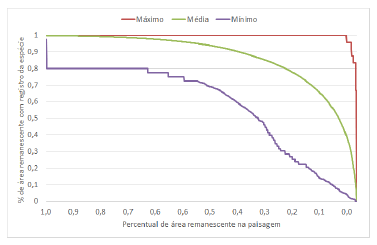
\includegraphics[width=0.8\linewidth]{imagens/figura01} 

}

\caption{Valores máximo, médio e mínimo dos percentuais de área remanescente com registro para o conjunto de espécies conforme avança a priorização (redução de área na paisagem).}\label{fig:01}
\end{figure}

\begin{longtable}[t]{>{}llrr}
\caption{\label{tab:1}Percentual de áreas com registros priorizado pelo Zonation na solução final.}\\
\toprule
Táxon & Espécie Ameaçada & A & B\\
\midrule
\em{Actitis macularius} & N & 591 & 86\\
\em{Anas discors} & N & 63 & 49\\
\em{Anas georgica} & N & 115 & 93\\
\em{Anas platalea} & N & 10 & 100\\
\em{Anas sibilatrix} & N & 7 & 100\\
\addlinespace
\em{Anas versicolor} & N & 127 & 95\\
\em{Anthracothorax nigricollis} & N & 1153 & 68\\
\em{Anthus correndera} & N & 20 & 100\\
\em{Arenaria interpres} & N & 233 & 96\\
\em{Attila phoenicurus} & N & 202 & 78\\
\addlinespace
\em{Bartramia longicauda} & N & 132 & 93\\
\em{Buteo platypterus} & N & 55 & 100\\
\em{Buteo swainsoni} & N & 52 & 100\\
\em{Calidris alba} & N & 233 & 96\\
\em{Calidris bairdii} & N & 8 & 100\\
\addlinespace
\em{Calidris fuscicollis} & N & 281 & 94\\
\em{Calidris himantopus} & N & 65 & 100\\
\em{Calidris melanotos} & N & 239 & 94\\
\em{Calidris minutilla} & N & 139 & 95\\
\em{Callonetta leucophrys} & N & 99 & 92\\
\addlinespace
\em{Casiornis fusca} & N & 384 & 48\\
\em{Catharus fuscescens} & N & 111 & 80\\
\em{Catharus minimus} & N & 8 & 100\\
\em{Catharus swainsoni} & N & 28 & 100\\
\em{Chaetura meridionalis} & N & 637 & 81\\
\addlinespace
\em{Charadrius falklandicus} & N & 17 & 100\\
\em{Charadrius modestus} & N & 41 & 100\\
\em{Charadrius semipalmatus} & N & 376 & 90\\
\em{Chionis albus} & N & 6 & 100\\
\em{Chlidonias niger} & N & 14 & 100\\
\addlinespace
\em{Chordeiles minor} & N & 115 & 90\\
\em{Cinclodes fuscus} & N & 17 & 100\\
\em{Coccyzus americanus} & N & 214 & 88\\
\em{Coccyzus melacoryphus} & N & 1024 & 67\\
\em{Contopus cooperi} & N & 51 & 100\\
\addlinespace
\em{Contopus virens} & N & 54 & 87\\
\em{Coscoroba coscoroba} & N & 64 & 100\\
\em{Cyanoloxia glaucocaerulea} & N & 341 & 76\\
\em{Dacnis nigripes} & N & 99 & 91\\
\em{Dendrocygna bicolor} & N & 221 & 90\\
\addlinespace
\em{Dolichonyx oryzivorus} & N & 30 & 100\\
\em{Elaenia chilensis} & N & 271 & 63\\
\em{Elaenia chiriquensis} & N & 552 & 57\\
\em{Elaenia parvirostris} & N & 683 & 70\\
\em{Elaenia spectabilis} & N & 735 & 67\\
\addlinespace
\em{Elanoides forficatus} & N & 866 & 72\\
\em{Empidonax alnorum} & N & 13 & 100\\
\em{Empidonomus varius} & N & 1939 & 59\\
\em{Falco peregrinus} & N & 384 & 86\\
\em{Florisuga fusca} & N & 813 & 71\\
\addlinespace
\em{Fluvicola albiventer} & N & 514 & 61\\
\em{Gelochelidon nilotica} & N & 82 & 100\\
\em{Griseotyrannus aurantioatrocristatus} & N & 498 & 64\\
\em{Harpagus diodon} & N & 466 & 85\\
\em{Heteronetta atricapilla} & N & 11 & 100\\
\addlinespace
\em{Hirundo rustica} & N & 492 & 80\\
\em{Hydropsalis parvulus} & N & 623 & 73\\
\em{Hymenops perspicillatus} & N & 113 & 97\\
\em{Ictinia mississippiensis} & N & 39 & 100\\
\em{Ictinia plumbea} & N & 1265 & 63\\
\addlinespace
\em{Inezia inornata} & N & 39 & 100\\
\em{Larus atlanticus} & N & 21 & 100\\
\em{Lathrotriccus euleri} & N & 1520 & 54\\
\em{Legatus leucophaius} & N & 792 & 73\\
\em{Lessonia rufa} & N & 23 & 100\\
\addlinespace
\em{Leucophaeus atricilla} & N & 62 & 100\\
\em{Limosa haemastica} & N & 79 & 98\\
\em{Lurocalis semitorquatus} & N & 426 & 78\\
\em{Micrococcyx cinereus} & N & 69 & 91\\
\em{Mimus triurus} & N & 165 & 92\\
\addlinespace
\em{Myiarchus swainsoni} & N & 1363 & 62\\
\em{Myiodynastes maculatus} & N & 2305 & 53\\
\em{Myiopagis viridicata} & N & 873 & 53\\
\em{Myiophobus fasciatus} & N & 1497 & 62\\
\em{Neochen jubata} & N & 84 & 100\\
\addlinespace
\em{Netta peposaca} & N & 64 & 95\\
\em{Numenius hudsonicus} & N & 149 & 99\\
\em{Nyctanassa violacea} & N & 156 & 97\\
\em{Oreopholus ruficollis} & N & 11 & 100\\
\em{Oxyura vittata} & N & 17 & 100\\
\addlinespace
\em{Pachyramphus polychopterus} & N & 1577 & 61\\
\em{Pachyramphus validus} & N & 1043 & 68\\
\em{Pandion haliaetus} & N & 597 & 83\\
\em{Pardirallus sanguinolentus} & N & 189 & 96\\
\em{Petrochelidon pyrrhonota} & N & 161 & 88\\
\addlinespace
\em{Phalaropus tricolor} & N & 61 & 100\\
\em{Pheucticus aureoventris} & N & 40 & 70\\
\em{Phoenicopterus chilensis} & N & 27 & 100\\
\em{Phytotoma rutila} & N & 10 & 100\\
\em{Piranga rubra} & N & 17 & 100\\
\addlinespace
\em{Pitangus sulphuratus} & N & 2929 & 50\\
\em{Platalea ajaja} & N & 743 & 76\\
\em{Plegadis chihi} & N & 358 & 80\\
\em{Pluvialis dominica} & N & 283 & 93\\
\em{Pluvialis squatarola} & N & 178 & 98\\
\addlinespace
\em{Podager nacunda} & N & 507 & 85\\
\em{Porphyrio martinicus} & N & 1056 & 68\\
\em{Progne chalybea} & N & 1793 & 62\\
\em{Progne elegans} & N & 14 & 100\\
\em{Progne subis} & N & 198 & 83\\
\addlinespace
\em{Progne tapera} & N & 1566 & 68\\
\em{Pseudocolopteryx acutipennis} & N & 13 & 100\\
\em{Pseudocolopteryx flaviventris} & N & 47 & 98\\
\em{Pygochelidon melanoleuca} & N & 108 & 85\\
\em{Pyrocephalus rubinus} & N & 1263 & 64\\
\addlinespace
\em{Riparia riparia} & N & 95 & 95\\
\em{Rostrhamus sociabilis} & N & 1165 & 66\\
\em{Rynchops niger} & N & 519 & 85\\
\em{Serpophaga griseicapilla} & N & 15 & 100\\
\em{Serpophaga munda} & N & 17 & 100\\
\addlinespace
\em{Setophaga petechia} & N & 30 & 97\\
\em{Setophaga ruticilla} & N & 16 & 100\\
\em{Setophaga striata} & N & 41 & 98\\
\em{Sporophila bouvreuil} & N & 398 & 66\\
\em{Sporophila caerulescens} & N & 1900 & 53\\
\addlinespace
\em{Sporophila cinnamomea} & N & 87 & 83\\
\em{Sporophila hypochroma} & N & 19 & 100\\
\em{Sporophila lineola} & N & 1422 & 57\\
\em{Stelgidopteryx ruficollis} & N & 2174 & 56\\
\em{Sterna hirundo} & N & 217 & 96\\
\addlinespace
\em{Sterna paradisaea} & N & 37 & 100\\
\em{Sterna trudeaui} & N & 69 & 100\\
\em{Sternula antillarum} & N & 53 & 100\\
\em{Sublegatus modestus} & N & 362 & 59\\
\em{Tachycineta leucopyga} & N & 36 & 100\\
\addlinespace
\em{Tersina viridis} & N & 1480 & 58\\
\em{Thalasseus acuflavidus} & N & 209 & 93\\
\em{Tringa flavipes} & N & 668 & 85\\
\em{Tringa melanoleuca} & N & 461 & 90\\
\em{Tringa semipalmata} & N & 114 & 99\\
\addlinespace
\em{Tringa solitaria} & N & 1134 & 70\\
\em{Turdus amaurochalinus} & N & 2353 & 50\\
\em{Turdus flavipes} & N & 645 & 66\\
\em{Turdus subalaris} & N & 506 & 71\\
\em{Tyrannus albogularis} & N & 670 & 63\\
\addlinespace
\em{Tyrannus melancholicus} & N & 2968 & 49\\
\em{Tyrannus savana} & N & 2053 & 57\\
\em{Tyrannus tyrannus} & N & 39 & 100\\
\em{Vireo altiloquus} & N & 26 & 100\\
\em{Vireo chivi} & N & 1225 & 70\\
\addlinespace
\em{Vireo olivaceus} & N & 10 & 100\\
\em{Xolmis coronata} & N & 6 & 100\\
\em{Calidris canutus} & CR & 98 & 100\\
\em{Limnodromus griseus} & CR & 90 & 100\\
\em{Calidris pusilla} & EN & 172 & 98\\
\addlinespace
\em{Thalasseus maximus} & EN & 120 & 100\\
\em{Amazona pretrei} & VU & 75 & 100\\
\em{Calidris subruficollis} & VU & 50 & 100\\
\em{Sporophila beltoni} & VU & 22 & 100\\
\em{Sporophila hypoxantha} & VU & 132 & 93\\
\addlinespace
\em{Sporophila melanogaster} & VU & 127 & 91\\
\em{Sporophila palustris} & VU & 64 & 100\\
\em{Sporophila ruficollis} & VU & 57 & 100\\
\em{Sterna dougallii} & VU & 33 & 100\\
\em{Sterna hirundinacea} & VU & 129 & 91\\
\addlinespace
\em{Tangara peruviana} & VU & 166 & 94\\
\bottomrule
\end{longtable}

\emph{Análises para as espécies migratórias não oceânicas, considerando um corte em 30\%.}\\
\emph{A = Número de células com registro pré-priorização}\\
\emph{B = \% de células com registro nas soluções finais}

\begin{enumerate}
\def\labelenumi{(\arabic{enumi})}
\setcounter{enumi}{1}
\tightlist
\item
  Para as Áreas Importantes para aves migratórias por expressiva concentração de indivíduos, foram levantadas 75 áreas (englobando 2.305 células) em 21 estados, totalizando uma área continental de 194.249 km\textsuperscript{2} aproximadamente, além das ilhas oceânicas. Cada área aqui elencada foi identificada, apresentada sua justificativa e sua fonte. Devido a uma disponibilidade desigual de informações, a maior parte das áreas levantadas apresenta ocorrência de espécies migratórias limícolas e costeiro-oceânicas, e são poucas as áreas regulares de rota, pousio, descanso, alimentação e reprodução para um volume expressivo de indivíduos florestais ou campestres. Assim, a área total considerando as Áreas Importantes por expressiva concentração de indivíduos e as elencadas pela modelagem no Zonation somou cerca de 346.262 Km\textsuperscript{2} (4.091 células), ou aproximadamente 4\% da superfície do Brasil.
\end{enumerate}

A seguir são apresentadas, por estado, as Áreas Importantes para aves migratórias por expressiva concentração de indivíduos:

Alagoas

\begin{itemize}
\tightlist
\item
  Área de Proteção Ambiental (APA) de Piaçabuçu: apresenta grande concentração de \emph{Tringa melanoleuca} (315 indivíduos), \emph{Tringa flavipes} (407), \emph{Arenaria interpres} (479), \emph{Calidris pusilla} (1.455) (Azevedo-Júnior \& Larrazábal 2011b).
\end{itemize}

Amapá

\begin{itemize}
\item
  Ilha do Parazinho: durante trabalho envolvendo anilhamento e análise de mudas, foram capturados mais de 700 indivíduos de aves limícolas, principalmente \emph{Actitis macularius}, \emph{Calidris pusilla} e \emph{Charadrius semipalmatus}, demonstrando que a área possui elevada concentração de indivíduos (Nascimento 1998);
\item
  Praia do Goiabal: importante área de concentração de aves limícolas migratórias, com registros de mais de 3.000 indivíduos de \emph{Calidris alba}, cerca de 2.400 de \emph{C. pusilla} e de 1.000 de \emph{Charadrius semipalmatus} (Rodrigues \& Carvalho 2011a).
\end{itemize}

Amazonas

\begin{itemize}
\item
  Reserva Extrativista Catuá-Ipixuna: registros de bandos de mais de 50 indivíduos de \emph{Calidris fuscicolis} e de \emph{Progne subis} na região (Andretti \& Costa 2011);
\item
  Remanso do Boto: bandos de mais de 50 indivíduos de \emph{Progne subis} (Almeida 2011);
\item
  Reserva de Desenvolvimento Sustentável Piagaçu-Purus: registros de reprodução de \emph{Rynchops niger} (Cintra et al.~2011);
\item
  Reserva de Desenvolvimento Sustentável Mamirauá: registros de reprodução de \emph{Rynchops niger} (SNA 2015);
  Bahia
\item
  Região de Cacha-Prego: é área de invernada de \emph{Sterna dougallii}. Os bancos de areia que ocorrem no local são vitais para que as aves possam descansar durante a invernada e alimentar-se em águas próximas (Lima \& Lima 2011);
\item
  Camamu: Esse banco de areia é utilizado também por \emph{Sterna dougallii} e \emph{S. hirundo}, formando concentrações de mais de 5.000 indivíduos (Lima et al.~2004);
\item
  Mangue Seco: localizada na APA do Litoral Norte da Bahia, as concentrações de \emph{Sterna dougallii} e \emph{S. hirundo} observadas são maiores, com mais de 10.000 indivíduos (P.C. Lima, comunicação pessoal - Lima \& Lima 2011).
\end{itemize}

Ceará

\begin{itemize}
\item
  Ilha Grande: ilha com cerca de 3.000 hectares, localizada no complexo estuarino dos rios Timonha (02°56'S, 41°17'W), Ubatuba. Concentração de ao menos 14 espécies de limícolas migratórias de origem Neártica (Charadriidae e Scolopacidae) em grandes concentrações de \emph{Pluvialis squatarola}, \emph{Arenaria interpres}, \emph{Numenius hudsonicus}, \emph{Charadrius semipalmatus}, \emph{Calidris pusilla} e \emph{Calidris minutilla} (Fedrizzi et al.~2016);
\item
  Banco dos Cajuais: em Icapuí, foi reconhecido em 2017 como sítio da Western Hemisphere Shorebird Reserves Network (WHSRN) por concentrar aves limícolas migratórias entre os quais mais de 1\% da população global de \emph{Calidris canutus rufa} e 1\% de \href{http://www.whsrn.org/banco-dos-cajuais}{\emph{Limnodromus griseus griseus}}, além de \emph{Charadrius semipalmatus}, \emph{Calidris pusilla}, \emph{Arenaria interpres}, \emph{Pluvialis squatarola} e \emph{Calidris alba} (Fedrizzi et al.~2016). Há o registro de reprodução de \emph{Charadrius wilsonia} (C.E. Fedrizzi - comunicação pessoal).
\end{itemize}

Espírito Santo

\begin{itemize}
\tightlist
\item
  Ilhas dos municípios de Vila Velha, Guarapari, Itapemirim e Marataízes: estas ilhas abrigam as maiores colônias reprodutivas de \emph{Thalasseus acuflavidus} no Atlântico Sul, correspondendo a mais de 1\% da população global da espécie. Foram estimados 10.000 indivíduos na Ilha Branca e de 10.000 a 13.000 indivíduos na Ilha Escalvada (Efe et al.~2000). Nas ilhas Itatiaia, há registros históricos de nidificação de \emph{Puffinus lherminieri} (Bencke et al.~2006), espécie migratória e ameaçada.
\end{itemize}

Maranhão

\begin{itemize}
\item
  Reentrâncias Maranhenses: correspondem à região da costa maranhense, que vai da divisa com o Pará até São Luís, recortada por várias reentrâncias e baías e com importantes unidades de conservação, como a APA das Reentrâncias Maranhenses e a RESEX Cururupu. Há registros de grandes concentrações de espécies, como, por exemplo, 26.000 indivíduos de \emph{Calidris pusilla} e 3.600 indivíduos de \emph{Limnodromus griseus} na Ilha do Cajual (Rodrigues 2000), 1.200 indivíduos de \emph{Limnodromus griseus} registrados em Ponta Seca e 700 indivíduos de \emph{Pluvialis squatarola}, em Croa Alta (Rodrigues \& Carvalho 2011c). No Golfão Maranhense, que inclui a Ilha de São Luís, destaca-se a praia do Raposo, onde Silva e Rodrigues (2015) encontraram densidade de 181 aves por hectare, com destaque para \emph{Calidris pusilla}, \emph{Tringa semipalmata} e \emph{Pluvialis squatarola}. Ainda merece ser mencionada a Ilha de Curupu que constitui o único local com registro de colônia reprodutiva de \emph{Sternula antillarum} no Brasil (Rodrigues et al.~2010);
\item
  Baixada Maranhense: também há grandes concentrações de aves limícolas migratórias, especialmente na Ilha dos Caranguejos, onde foram registradas grandes concentrações de \emph{Calidris pusilla} (cerca de 35.000 indivíduos) e \emph{Calidris canutus} (em torno de 7.000 indivíduos) (Carvalho \& Rodrigues 2011). É um dos poucos lugares do Brasil onde há numerosas concentrações de \emph{Porphyrio martinicus} (frango d'água-azul), um ralídeo de hábitos migratórios que sofre intensa pressão de caça na região (De Luca et al.~2009). Também ocorrem concentrações de \emph{Tringa flavipes} (cerca de 320 indivíduos registrados) (Roth \& Scott 1987) e \emph{Tringa semipalmata} (mais de 1.500 indivíduos) (Carvalho \& Rodrigues 2011).
\end{itemize}

Mato Grosso

\begin{itemize}
\item
  Chapada dos Guimarães: área de ocorrência das espécies migratórias \emph{Ictinia mississippiensis} e \emph{Rostrhamus sociabilis}, sendo que esse último foi observado em grupos de mais de 2.500 indivíduos (P.P. Amaral -- observação pessoal);
\item
  RPPN Sesc Pantanal: importante área de alimentação e reprodução para \emph{Rynchops niger} (Mariano-Jelicich \& Madrid 2014).
\end{itemize}

Mato Grosso do Sul

\begin{itemize}
\tightlist
\item
  Região de Nhecolândia e Paiaguás: registrada a ocorrência de bandos com centenas de indivíduos de \emph{Tringa melanoleuca} e \emph{Tringa flavipes} (Nunes et al.~2011).
\end{itemize}

Pará

\begin{itemize}
\tightlist
\item
  Reentrâncias Paraenses: juntamente com as Reentrâncias Maranhenses, abriga mais de 90\% da população de diversas espécies de aves limícolas migratórias do Brasil, como: \emph{Arenaria interpres, Calidris pusilla, Limnodromus griseus, Numenius hudsonicus, Pluvialis squatarola e Tringa semipalmata}. Há registros de grandes concentrações para algumas delas: até 6.000 indivíduos de \emph{Calidris pusilla}, 1.200 indivíduos de \emph{P. squatarola}, 300 indivíduos de \emph{Limnodromus griseus} e a mesma quantidade de \emph{Numenius hudsonicus} (Rodrigues \& Carvalho 2011b).
\end{itemize}

Paraná

\begin{itemize}
\item
  O Parque Municipal de Barigui: abriga grupos numerosos de \emph{Tringa flavipes} em certas épocas do ano, havendo registro de quase 500 indivíduos (Deconto \& Aurélio-Silva 2011);
\item
  O Parque Nacional da Ilha dos Currais e Ilhas da Figueira e Itacolomi: área de pouso e reprodução de espécies migratórias como \emph{Sterna hirundinacea} (100 casais) e \emph{Thalasseus acuflavidus} (100 casais) (Krul 2004). É reconhecido como IBA (BR209) (Bencke et al.~2006);
\item
  Região dos Campos Gerais: utilizada por \emph{Petrochelidon pyrrhonota} durante a invernada, havendo bandos de até 3.000 indivíduos (Santos 2011).
\end{itemize}

Pernambuco

\begin{itemize}
\tightlist
\item
  Ilha da Coroa do Avião: uma ilhota situada no Canal de Santa Cruz é uma área importante para a migração de \emph{Calidris alba} (Lyra-Neves et al.~2004) com registros de mais de 400 indivíduos utilizando os bancos de areia da ilha (Cardoso \& Nascimento 2007).
\end{itemize}

Rio de Janeiro

\begin{itemize}
\tightlist
\item
  Região do município de Quissamã, incluindo o PARNA da Restinga de Jurubatiba: se destaca por abrigar grandes concentrações (mais de 6.000 indivíduos) de aves limícolas principalmente representadas por \emph{Calidris fuscicollis}, \emph{Calidris alba} e \emph{Tringa flavipes} (Tavares et al.~2015).
\end{itemize}

Rio Grande do Norte

\begin{itemize}
\item
  Salina Diamante Branco: área de concentração de algumas espécies de aves limícolas, como \emph{Calidris pusilla} com cerca de 1.500 indivíduos, \emph{Tringa flavipes} com mais de 400 indivíduos e \emph{Tringa melanoleuca} representada por mais de 300 indivíduos (Azevedo-Júnior \& Larrazábal 2011a);
\item
  Complexo Litorâneo da Bacia Potiguar: quatro localidades importantes por concentrações de aves migratórias: as salinas de Macau (120 km\^{}\textsuperscript{2}) e de Galinhos (50 km\textsuperscript{2}), a área em torno de Soledade (Macau; 15 km\textsuperscript{2}) e a lagoa Lagamar (Carnaubais e Porto de Mangue; 2 km\textsuperscript{2}). Destacam-se os registros de grupos de mais de 1.000 indivíduos de \emph{Limnodromus griseus}, 2.800 indivíduos de \emph{Calidris pusilla} e mais de 400 indivíduos de \emph{Tringa flavipes} e \emph{Tringa melanoleuca} (Irusta \& Sagot-Martin 2011).
\end{itemize}

Rio Grande do Sul

\begin{itemize}
\item
  Área de Proteção Ambiental (APA) do Ibirapuitã: área de reprodução de \emph{Sporophila palustris} que, além de migratória, é espécie ameaçada (Maurício et al.~2014);
\item
  Região dos Banhados e Cordões Litorâneos: especialmente no Banhado do Maçarico, ocorre a maior população reprodutiva de \emph{Sporophila palustris} do Brasil (entre 200 e 300 indivíduos -- cerca de 10\% da população global estimada), espécie migratória e ameaçada (Mauricio et al.~2014);
\item
  Estuário da Laguna dos Patos: área de maior concentração regular de \emph{Calidris subruficollis} no Brasil (Lanctot et al.~2002). Essa espécie, além de migratória, é ameaçada de extinção (MMA 2014). Há também grandes concentrações de \emph{Tringa flavipes} e \emph{Pluvialis dominica}, chegando a reunir mais de 400 (Dias et al.~2011) e 500 indivíduos (Lanctot et al.~2002), respectivamente;
\item
  Banhado de São Donato: área reprodutiva de \emph{Sporophila palustris} (Mauricio et al.~2014), de Sporophila cinnamomea (Krügel et al.~2014) e de \emph{Rostrhamus sociabilis} (Bencke et al.~2006);
\item
  Estação Ecológica (ESEC) do Taim: abriga as maiores populações conhecidas de \emph{Coscoroba coscoroba} (cerca de 1.500 indivíduos), e há também registro de centenas de \emph{Calidris subruficollis} (espécie migratória e ameaçada) durante o verão austral (Lanctot et al.~2002) e é área de reprodução de cerca de 12.000 indivíduos de \emph{Plegadis chihi} (Matheu et al.~2014);
\item
  Campos da Região de Bagé: representam uma das poucas áreas reprodutivas de \emph{Sporophila cinnamomea} no Brasil (Krügel et al.~2014);
\item
  Parque Estadual do Espinilho: área reprodutiva de \emph{Sporophila palustris} (Mauricio et al.~2014).
\item
  Parque Nacional da Lagoa do Peixe: reconhecido desde 1990 como sítio da \emph{Western Hemisphere Shorebird Reserves Network (WHSRN)} de importância internacional por abrigar mais de 10\% da população global de \emph{Limosa haemastica} e \emph{Calidris canutus rufa}, além de mais de 1\% da população de outras quatro espécies: \emph{Calidris subruficollis}, \emph{Pluvialis dominica}, \emph{Calidris fuscicollis} e \href{https://www.whsrn.org/lagoa-do-peixe}{\emph{Calidris alba}} (Morrison et al.~2006). Ocorrem neste parque mais de 20 espécies de aves limícolas de origem Neártica, três de migrantes austrais e cinco que se reproduzem no local. Além destas, também ocorrem anatídeos migratórios, como \emph{Anas georgica}, flamingos e cegonhas, entre outros (Nascimento 1995). A área é também utilizada por grandes grupos de \emph{Sterna hirundo}, chegando a formar concentrações de 12.000 a 14.000 indivíduos (Bencke et al.~2006). No trecho de praia oceânica na porção norte do parque há registros de grandes concentrações de aves migratórias, com destaque para \emph{Calidris alba} (até 3.100 indivíduos), \emph{Calidris canutus rufa} (até 1.900) e \emph{Calidris fuscicollis} (até 3.400) (Fedrizzi 2008; CEMAVE/PNL - monitoramento 2012-2018, em preparo). Já na região lagunar, próxima à barra, foram registrados mais de 6.000 indivíduos de \emph{Calidris fuscicollis} em abril de 2005 e mais de 14.000 em novembro 2006 (Fedrizzi 2008). No mesmo local, foram registrados mais de 1.000 indivíduos de \emph{Limosa haemastica} nos anos '80 (Harrington et al.~1986) e 300 indivíduos em 2005 (Fedrizzi 2008). Também é nas áreas lagunares que se concentra \emph{Tringa flavipes} (c.~2.500 indivíduos) (Gonçalves 2009). Nos campos úmidos ao redor da Lagoa do Peixe é que \emph{Pluvialis dominica} e \emph{Calidris subruficollis} têm um de seus principais sítios de invernada em escala mundial (Lanctot et al.~2002, Morrison et al.~2006). Próximo ao limite sul do Parque, foram registradas as maiores concentrações de \emph{Calidris canutus rufa}: 11.000 indivíduos em 1982 (Harrington et al.~1986), 7.000 em 1984 (Resende 1988) e 5.200 em 2005 (Fedrizzi 2008);
\item
  Reserva Biológica (REBIO) do Mato Grande e a várzea do Canal de São Gonçalo: são importantes áreas reprodutivas de \emph{Sporophila palustris} (Mauricio et al.~2014).
\item
  Região nordeste do Rio Grande do Sul: região dos campos de cima da serra dos municípios de Vacaria, Bom Jesus e São José dos Ausentes, é área de reprodução de \emph{Sporophila beltoni} (Repenning \& Fontana 2013).
\item
  Reserva da Capitulina: Na área conhecida localmente como Reserva da Capitulina, em fevereiro de 2019, foi observado um grande número de territórios de patativa-tropeira (\emph{Sporophila beltoni}) em habitats com boa continuidade (M. Repenning \& C. Fontana, comunicação pessoal).
\item
  Foz do rio dos Touros: Contempla muitos territórios reprodutivos de patativa tropeira (\emph{Sporophila beltoni}). Presença de outras espécies ameaçadas e especialistas de campo (\emph{S. hypoxantha}, \emph{S. melanogaster}) (M. Repenning \& C. Fontana -- comunicação pessoal).
\item
  Ninhos/Vacaria: Este conjunto de pequenas propriedades é uma área importante para reprodução de \emph{Sporophila beltoni} (M. Repenning \& C. Fontana -- comunicação pessoal).
\end{itemize}

Santa Catarina

\begin{itemize}
\item
  Região dos Campos de Cima da Serra: ocorrem populações reprodutivas de \emph{Sporophila hypoxantha} (Franz \& Fontana 2013).
\item
  Lages: é área de reprodução de \emph{Sporophila beltoni} (Repenning \& Fontana 2013).
\item
  Região dos Campos de Água Doce: abriga população reprodutiva isolada de \emph{Sporophila melanogaster}, espécie migratória, ameaçada e endêmica do Brasil, que possui toda sua população reprodutiva confinada aos campos de altitude de Santa Catarina e do Rio Grande do Sul (Serafini 2014).
\item
  Município de Urupema: existe uma área de importante concentração de \emph{Amazona pretrei} no período não-reprodutivo, a partir do mês de maio, quando é registrada a agregação de milhares de indivíduos (Schunck et al.~2011);
\item
  Ilhas marinhas costeiras da Deserta (REBIO Arvoredo), Moleques do Sul (Parque Estadual do Tabuleiro), Santana de Dentro e Santana de Fora (APA da Baleia Franca): constituem áreas de pouso e reprodução de \emph{Sterna hirundinacea} e \emph{Thalasseus acuflavidus} (até 1.200 de ambas as espécies) (Branco 2004).
\item
  Coxilha Rica: Principal área reprodutiva de \emph{Sporophila beltoni}. Destacando-se a área a oeste do rio Lava Tudo, localidade Coxilha Rica com co-ocorrência de \emph{S. hypoxantha} e \emph{S. melanogaster}. O lado leste do rio, localidade de Estância do Meio, contempla número muito significativo de territórios reprodutivos de S. beltoni (M. Repenning \& C. Fontana -- comunicação pessoal).
\end{itemize}

São Paulo

\begin{itemize}
\item
  Arquipélago de Alcatrazes: importante área reprodutiva de espécies marinhas e migratórias como Sterna hirundinacea. Abriga (ilha dos Amigos e laje das Trinta-réis) uma das poucas colônias reprodutivas de \emph{Thalasseus maximus} no Brasil, com cerca de 60 pares (Campos et al.~2004, Bencke et al.~2006);
\item
  Ilha Bela: área de reprodução de \emph{Thalasseus maximus} (ilha da Prainha) e \emph{Sterna hirundinacea} (Campos et al.~2004);
\item
  Laje de Santos: área de reprodução de \emph{Thalasseus maximus} e \emph{Sterna hirundinacea} (Campos et al.~2004);
\item
  Ilhote das Gaivotas: área de reprodução de \emph{Thalasseus maximus} (Campos et al.~2004);
\item
  Laje da Conceição: área de reprodução de \emph{Thalasseus maximus} (Campos et al.~2004);
\item
  Castilho: em Cananéia. Área de reprodução de \emph{Sterna hirundinacea} (60 adultos entre 1988 e 1990, Olmos et al.~1995 apud Campos et al.~2004);
\item
  Ilha da Figueira (divisa estado do Paraná): área de reprodução de \emph{Sterna hirundinacea} (100 ninhos em 2000/2001)
\item
  Bacia hidrográfica do reservatório Guarapiranga: compreende todas as APP da bacia, incluindo o Parque Praia do Sol, as várzeas e a foz do rio Embu-Mirim, o Parque Ilha dos Eucaliptos e o Parque Ecológico do Guarapiranga, foram registrados grupos de até 300 indivíduos de \emph{Tringa melanoleuca} e de até 200 de \emph{Tringa flavipes} (Schunck 2011).
\end{itemize}

Sergipe

\begin{itemize}
\item
  Estuário do rio Sergipe: há concentração de vários Charadriiformes migratórios, destacando se o registro de cerca de 2.200 indivíduos de \emph{Charadrius semipalmatus} e 200 indivíduos de \emph{Numenius hudsonicus}. Na região também há registro de \emph{Falco peregrinus} e de \emph{Sterna hirundo}, com bandos de até 100 indivíduos acompanhando barcos de pesca (Sousa 2011a);
\item
  Complexo do estuário dos rios Piauí, Fundo e Real: um local importante para o descanso e alimentação das aves migratórias provenientes, em sua grande maioria, do Hemisfério Norte. Já foram registradas 14 espécies migratórias, destacando-se concentrações de mais de 300 \emph{Numenius hudsonicus} (Sousa 2011b);
\item
  Estuário do rio Vaza-Barris: este estuário é uma área importante para o descanso e alimentação das aves migratórias, havendo registro de ao menos 14 espécies, destacando-se o registro de 277 \emph{Calidris alba} e cerca de 300 \emph{Sterna hirundo} (Sousa 2011c);
\item
  Praias de Aracaju: abrigam concentrações de até 400 indivíduos de \emph{Calidris alba} (Almeida 2004, Almeida 2010, Almeida \& Ferrari 2011).
\end{itemize}

Tocantins

\begin{itemize}
\item
  APA da Ilha do Bananal: foram registrados bandos de cerca de 500 indivíduos de \emph{Buteo swainsoni} (Dornas \& Pinheiro 2011);
\item
  Parque Estadual do Cantão: além de algumas espécies migratórias de Charadriiformes, foi registrado um bando de \emph{Progne subis}, o qual foi estimado entre 5.000 e 8.000 indivíduos (Pinheiro \& Dornas 2009). Essa espécie de andorinha parece ser fiel ao sítio de invernada, sendo observada em anos consecutivos na região (Dornas \& Pinheiro 2011).
\end{itemize}

Ilhas oceânicas

As ilhas oceânicas são via de regra áreas extremamente importantes para a avifauna marinha e migratória. O arquipélago de Fernando de Noronha (PE) e de Abrolhos (BA), o Atol das Rocas (RN) e as ilhas de Trindade e Martim Vaz (ES) são pontos de pousio, descanso, alimentação e reprodução críticos. \emph{Onychoprion fuscatus} nidifica em todas estas ilhas oceânicas. O Arquipélago de Fernando de Noronha é, atualmente, o único local reprodutivo de \emph{Puffinus lherminieri} no Brasil. \emph{Pterodroma arminjoniana}, no Atlântico Sul, reproduz apenas em Trindade e Martim Vaz e o Atol das Rocas destaca-se por ser área com a maior concentração de aves marinhas em nidificação no Brasil. Alguns migrantes também utilizam a área do Atol para repouso e alimentação: \emph{Pluvialis squatarola}, \emph{Charadrius semipalmatus}, \emph{Arenaria interpres}, \emph{Numenius hudsonicus} e \emph{Limnodromus griseus} (Alves et al.~2004, Sick 1997, Fonseca-Neto 2004, Bencke et al.~2006).

\begin{figure}

{\centering 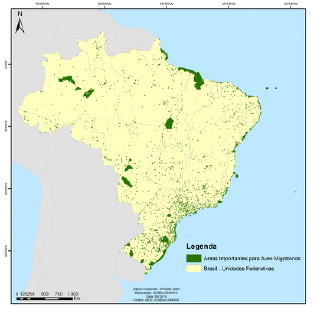
\includegraphics[width=0.8\linewidth]{imagens/figura02} 

}

\caption{Áreas Importantes para Aves Migratórias (áreas regulares de rota, pousio, descanso, alimentação e reprodução) no Brasil.}\label{fig:02}
\end{figure}

\hypertarget{mapa-ameacadas}{%
\section{Mapa de registros de aves ameaçadas de extinção}\label{mapa-ameacadas}}

A seguir é apresentado o mapa de registros de aves ameaçadas de extinção no Brasil listadas na Portaria 444, do Ministério do Meio Ambiente, de 17 de dezembro de 2014.

\hypertarget{contexto}{%
\subsection{Contexto}\label{contexto}}

São formalmente reconhecidos como ameaçados de extinção, 236 táxons de aves dentre as 1.903 espécies avaliadas em 2014. Três espécies já foram consideradas extintas em território brasileiro: o maçarico-esquimó (\emph{Numenius borealis}), o peito-vermelho-grande (\emph{Sturnella defilippii}), e a arara-azul-pequena (\emph{Anodorhynchus glaucus}) e três táxons endêmicos do Brasil foram considerados extintos globalmente: o gritador-do-nordeste (\emph{Cichlocolaptes mazarbarnetti}), o limpa-folha-do-nordeste (\emph{Philydor novaesi}) e o caburé-de-pernambuco (\emph{Glaucidium mooreorum}).

As principais ameaças às aves brasileiras, apontadas durante o processo de avaliação, foram o desmatamento e a fragmentação de habitat oriundos de atividades antrópicas, especialmente aquelas relacionadas às atividades agropecuárias e à expansão urbana. Outras ameaças relevantes são as queimadas e a captura de animais, seja para consumo seja para o comércio ilegal para servirem como animais de estimação.

\hypertarget{metodos2}{%
\subsection{Métodos}\label{metodos2}}

Os dados utilizados foram obtidos no Atlas de \href{http://ara.cemave.gov.br}{Registros de Aves Brasileiras - ARA} sob responsabilidade do ICMBio/CEMAVE. Esses dados são uma combinação de dados históricos compilados de publicações científicas e dados fornecidos por pesquisadores e colaboradores. Também foram utilizados dados disponibilizados pelo sítio de Internet \href{http://www.wikiaves.com}{Wikiaves - Enciclopédia das Aves do Brasil}. A lista de espécies seguiu a nomenclatura proposta pelo Comitê Brasileiro de Registros Ornitológicos - CBRO (Piacentini et al.~2015).

Da mesma forma que para o relatório de rotas e áreas de concentração de aves migratórias no Brasil, os registros foram plotados em uma grade com células quadradas de 5' de lado, aproximadamente 9,2 km no equador, e todas aquelas com registros foram recrutadas para a composição do mapa.

\hypertarget{resultados2}{%
\subsection{Resultados}\label{resultados2}}

Todos os estados brasileiros apresentam registros de espécies de aves ameaçadas. Contudo da mesma forma que observado nas áreas priorizadas para as aves migratórias, o padrão ainda um tanto disperso das áreas traduz as lacunas de conhecimento sobre a distribuição e ocorrência das espécies de aves brasileiras. A despeito disto é possível observar alguns padrões: o adensamento de áreas com espécies ameaçadas nas regiões Nordeste, Sudeste e Sul, e, em especial, nas zonas litorâneas, as quais, historicamente, são áreas com ocupação humana bastante densa (Figura \ref{fig:03}).

\begin{figure}

{\centering 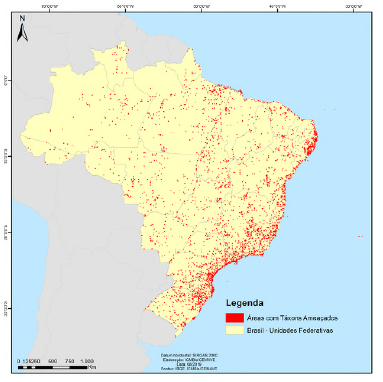
\includegraphics[width=0.8\linewidth]{imagens/figura03} 

}

\caption{Áreas com registros de ocorrência de aves ameaçadas conforme Portaria MMA 444/14.}\label{fig:03}
\end{figure}

Este mapa busca contribuir para o atendimento do inciso VII do Art. 3º, da Resolução Conama N° 462, de 24 de julho de 2014, no que tange às espécies ameaçadas. Contudo, não é um produto que se esgota em sim mesmo, possui limitações óbvias dadas pela dimensão continental do país e pelo incipiente conhecimento sobre nossa biodiversidade. Assim sendo, constitui-se apenas uma ferramenta de subsídio ao gestor ou consultor ambiental. É imprescindível que todo processo de licenciamento busque avaliar a presença ou potencial presença local de espécies ameaçadas no tempo presente.

\hypertarget{cons-finais}{%
\section{Considerações finais}\label{cons-finais}}

O planejamento sistemático de priorização de áreas ocupadas por espécies sensíveis a determinado tipo de empreendimento não é um trabalho que se encerra. Além das óbvias evoluções metodológicas e tecnológicas que nos permitem refinar os produtos, é importante esclarecer que o estudo das migrações é ainda incipiente no Brasil e que a dinâmica das migrações varia de acordo com mudanças em muitos parâmetros e em todas as escalas, desde mudanças climáticas globais, passando por flutuações populacionais e chegando a alterações em pequenos sítios na rota migratória. Sendo assim, a priorização precisa ser constantemente revisada para que novos cenários sejam considerados e para que o planejamento esteja condizente com a realidade atual.

O aporte de críticas ao processo aqui utilizado e de novas informações para alimentar esses modelos é muito bem-vindo. Sabemos que este trabalho é resultado do empenho de muitas pessoas, mesmo que indiretamente, e esperamos que a colaboração entre aqueles que detêm conhecimento sobre nossa biodiversidade e as instituições que trabalham por sua conservação seja cada vez maior, a fim de que possamos melhor atuar para garantir o bem comum.

\hypertarget{agradecimentos}{%
\section{Agradecimentos}\label{agradecimentos}}

Agradecemos ao professor Dr.~Rafael Luís Galdini Raimundo e a Elliott Victor de Sousa Chaves, Murilo Sérgio Arantes e Rosana Figueiredo.

\hypertarget{referencias}{%
\section{Referências bibliográficas}\label{referencias}}

Able, K.P. 1999. Gatherings of angel: migrating birds and their ecology. Ithaca, Cornell University Press, 193p.
Alerstam, T. 1990. Bird Migration. Cambridge, Cambridge University Press, 422p.

Almeida, B.J.M. 2004. Estrutura da população e aspectos ecológicos das aves da praia da Atalaia e do Mangue da Coroa do Meio. Relatório Técnico. Iniciação à Pesquisa PIBIC/CNPq. 34p.

Almeida, B.J.M. 2010. As aves limícolas migratórias nas praias de Aracaju: avaliação da influência antrópica e contribuição para ações de desenvolvimento costeiro. Dissertação de Mestrado. Aracaju, Universidade Federal de Sergipe. 90p.

Almeida, R.A.M. 2011. Remanso do Boto, p.68-73. In: Valente, R.; Silva, J.M.C.; Straube, F.C. \& Nascimento, J.L.X. (org). Conservação de aves migratórias neárticas no Brasil. Belém, Conservation International, 406p.

Almeida, B.J.M. \& Ferrari, S.F. 2011. Migratory Shorebirds at a stopover site in Northeastern Brazil: Habitat Use and Anthropogenic Impacts, p.22-23. In: 4th Meeting of Western Hemisphere Shorebird Group. Abstracts. Canadá, Simon Fraser University. 137p.

Alves, V.S.; Soares, A.B.A.; Couto, G.S.; Efe, M.A.~\& Ribeiro, A.B.B. 2004. Aves marinhas de Abrolhos, p.213-232. In: Branco, J.O. (org). Aves marinhas e insulares brasileiras: bioecologia e conservação. Itajaí, Editora Univali, 266p.

Andretti, C.B. \& Costa, T.V.V. 2011. Reserva Extrativista Catuá-Ipixuna, p.46-49. T: Valente, R.; Silva, J.M.C.; Straube, F.C. \& Nascimento, J.L.X. (org). Conservação de aves migratórias neárticas no Brasil. Belém, Conservation International, 406p.

ANEEL- Agência Nacional de Energia Elétrica. 2015. Centrais Geradoras Eolioelétricas - EOL. Sistema de Informações Georreferenciadas do Setor Elétrico - SIGEL. Disponível em: \textless{}\url{http://} sigel.aneel.gov.br/sigel.html\textgreater. Acesso em: 15/09/2015.

Antas, P.T.Z. 1983. Migration of Neartic shorebirds (Charadriidae and Scolopacidae) in Brazil -- flyways and their different seasonal use. Wader Study Group Bulletin 39(1): 52-56.

Antas, P.T.Z. 1987. Migração de aves no Brasil, p.153-187. Anais do II Encontro Nacional de Anilhadores de Aves. Rio de Janeiro: Editora UFRJ.

Atienza, J.C.; Fierro, I.M.; Infante, O. \& Valls, J. 2008. Directrices para la evaluación del impacto de lós parques eólicos en aves y murciélagos. (version 1.0). SEO/Birdlife, Madrid. 53p.

Azevedo-Júnior, S.M. \& Larrazábal, M.E. 2011a. Salina Diamante Branco, p.146-149. In: Valente, R.; Silva, J.M.C.; Straube, F.C. \& Nascimento, J.L.X. (org). Conservação de aves migratórias neárticas no Brasil. Belém, Conservation International, 406p.

Azevedo-Júnior, S.M. \& Larrazábal, M.E. 2011b. Pontal do Peba, p.159-162. In: Valente, R.; Silva, J.M.C.; Straube, F.C. \& Nascimento, J.L.X. (org). Conservação de aves migratórias neárticas no Brasil. Belém, Conservation International, 406p.

Barclay, R.M.R.; Baerwald, E.F. \& Gruver, J.C. 2007. Variation in bat and bird fatalities at wind energy facilities: assessing the effects of rotor size and tower height. Journal of Zoology 85: 381-387.

Barrios, L. \& Rodríguez, A. 2004. Behavioural and environmental correlates of soaring bird mortality at onshore wind turbines. Journal of Applied Ecology 41: 72-81.

Bencke, G.A.; Mauricio, G.N.; Develey, P.F. \& Goerck J.M. 2006. Áreas importantes para a Conservação das aves no Brasil: Parte I - Estados do Domínio da Mata Atlântica. São Paulo, SAVE Brasil. 494p.

Bernardino, J.; Bevanger, K.; Barrientos, R.; Dwyer, J.F.; Marques, A.T.; Martins, R.C.; Shaw, J. M.; Silva, J.P. \& Moreira, F. 2018. Bird collisions with power lines: state of the art and priority areas for research. Biological Conservation 222: 1-13.

Bevanger, K. 1994. Bird interactions with utility structures: collision and electrocution, causes and mitigating measures. Ibis 136: 412--425.

Bevanger, K. 1998. Biological and conservation aspects of bird mortality caused by electricity power lines: a review. Biological Conservation 86: 67-76.

Biasotto, L.D.; Barcelos-Silveira, A.; Agne, C.E.Q. \& Kindel, A. 2013. Comportamento de voos de aves em resposta ao uso de sinalizadores em linhas de transmissão de energia elétrica. Iheringia, ser. Zoo., 107: e2017047.
BirdLife International. 2014a. Migratory Birds and Flyways. Disponível em \url{http://www.birdlife.org/worldwide/programmes/migratory-birds-and-flyways}. Acesso em: 20/3/2014.

BirdLife International. 2014b. Important Bird and Biodiversity Areas: A global network for conserving nature and benefiting people. Cambridge, UK: BirdLife International. 26p.

Paton, S.R; Smallie J.; Pearson A. \& Ramalho, R. 2017. Wind energy's impacts on birds in South Africa: A preliminary review of the results of operational monitoring at the first wind farms of the Renewable Energy Independent Power Producer Procurement Programme in South Africa. BirdLife South Africa Occasional Report Series No.~2. BirdLife South Africa, Johannesburg, South Africa. 28p.

Branco, J.O. 2004. Aves Marinhas das Ilhas de Santa Catarina. In: Branco, J.O. (org). Aves marinhas e insulares brasileiras: biologia e conservação. Itajaí, Editora Univali. 266p.

Brasil. 2014. Ministério das Minas e Energia. Resenha Energética Brasileira: exercício de 2014. Brasília. 32p.
Caixa (Caixa Econômica Federal). 2016. Boas Práticas Socioambientais - Setor de Energia Elétrica. Gerência Nacional de Sustentabilidade e Responsabilidade Socioambiental \& Origami Consultoria em Gestão de Negócios Sustentáveis LTDA. 18p.

Campos, F.P.; Paludo, D.; Faria, P.J. \& Martuscelli, P. 2004. Aves Insulares Marinhas, residentes e migratórias do litoral do estado de São Paulo, p.57-82. In: Branco, J.O. (org.). Aves marinhas e insulares brasileiras: biologia e conservação. Itajaí, Editora Univali. 266 p.~

Cardoso, T.A.L. \& Nascimento, J.L.X. 2007. Avaliação de atividades turísticas prejudiciais à permanência das aves migratórias na Coroa do Avião, Pernambuco, Brasil. Ornithologia 2(2): 170-177.

Carrete, M.; Sánchez-Zapata, J.A.; Benítez, J.R.; Lobón, M.; Donázar, J.A. 2009. Large scale risk-assessment of wind farms on population viability of a globally endangered long-lived raptor. Biological Conservation 142: 2954-2961.

Carvalho, D.L. \& Rodrigues, A.A.F. 2011. Spatial and temporal distribution of migrant shorebirds (Charadriiformes) on Caranguejos Island in the Gulf of Maranhão, Brazil. Revista Brasileira de Ornitologia 19(4): 486-492.

Castro, C. \& Myers, J.P. 1987. Ecología y conservación del playero blanco (Calidris alba) en el Peru. Boletin Lima 52: 47-61.

Cintra, R.; Kasecker, T. \& Melo, A.V. 2011. Reserva de Desenvolvimento Sustentável Piagaçu-Purus, p.50-54. In: Valente, R.; Silva, J.M.C.; Straube, F.C. \& Nascimento, J.L.X. (org). Conservação de aves migratórias neárticas no Brasil. Belém, Conservation International, 406p.
Cornell University. 2014. All About Birds: Migration. Disponível em \textless{}\url{http://www}. birds.cornell.edu/AllAboutBirds/studying/ migration/\textgreater{} Acesso em: 20/3/2014.

De Luca, A.C.; Develey, P.F.; Bencke, G.A. \& Goerck, J.M. (orgs.). 2009. Áreas importantes para a conservação das aves no Brasil. Parte II -- Amazônia, Cerrado e Pantanal. São Paulo, SAVE Brasil, 382p.

Deconto, L.R. \& Aurélio-Silva, M. 2011. Parque Municipal do Barigüi, p.288-291. In: Valente, R.; Silva, J.M.C.; Straube, F.C. \& Nascimento, J.L.X. (org). Conservação de aves migratórias neárticas no Brasil. Belém, Conservation International. 406p.

Dias, R.A.; Gianuca, D.; Gianuca, A.T.; Gomes-Junior, A.; Chiaffitelli, R. \& Ferreira, W.L.S. 2011. Estuário da Lagoa dos Patos, p.335-341. In: Valente, R.; Silva, J.M.C.; Straube, F.C. \& Nascimento, J.L.X. (org). Conservação de aves migratórias neárticas no Brasil. Belém, Conservation International. 406p.

Dornas, T. \& Pinheiro, R.T. 2011. Ilha do Bananal e Planície do Cantão, p.111-115. In: Valente, R.; Silva, J.M.C.; Straube, F.C. \& Nascimento, J.L.X. (org). Conservação de aves migratórias neárticas no Brasil. Belém, Conservation International. 406p.

Drewitt, A.L. \& Langston, R.H.W. 2006. Assessing the impacts of wind farms on birds. Ibis 148: 29-42.
Drewitt, A.L. \& Langston, R.H.W. 2008. Collision effects of wind-power generators and other obstacles on birds. Annals of the New York Academy of Sciences 1134: 233-266.
Dwyer, J.; Pandey, A.K.; McHale L.A. \& Harness, R. 2019.\\
Near-ultraviolet light reduced Sandhill Crane collisions with a power line by 98\%. The Condor Ornithological Applications. Volume XX, pp 1-10.

Efe, M.A; Nascimento, J.L.X; Nascimento, I.L.S. \& Musso, C. 2000. Distribuição e Ecologia reprodutiva de Sterna sandvicensis eurygnatha no Brasil. Melopsittacus 3(3): 110-121.

EPHC (Environment Protection and Heritage Council). 2010. National Wind Farm Development Guidelines -- Draft. Environment Protection and Heritage Council. Australia, Adelaide, 198p.

Erickson, W.P.; Johnson, G.D.; Strickland, M.D.; Young, D.P.; Sernka, K.J. \& Good, R.E. 2001. Avian collisions with wind turbines: a summary of existing studies and comparisons to other sources of avian collision mortality in the United States. National Wind Coordinating Committee. 62p.

Evans, W.R., Akashi, Y., Altman, N.S. \& Manville, A.M., 2007. Response of night-migrating songbirds in cloud to colored and flashing light. North American Birds 60: 476--488.

Fedrizzi, C.E. 2008. Distribuição, abundância e ecologia alimentar de aves limícolas (Charadriiformes: Charadrii e Scolopaci) na zona costeira do Rio Grande do Sul, Brasil. Fundação Universidade de Rio Grande, Rio Grande. 176f.
Fedrizzi, C.E.; Carlos, C.J.; Campos, A.A. 2016. Annual patterns of abundance of Nearctic shorebirds and their prey at two estuarine sites in Ceará, NE Brazil, 2008-2009. Wader Study 123: 122-135.

Fonseca-Neto, F.P. 2004. Aves marinhas da ilha Trindade, p.119-146. In: Branco, J.O. (org.). Aves marinhas e insulares brasileiras: biologia e conservação. Itajaí, Editora Univali. 266p.

Franz, I. \& Fontana, C.S. 2013. Breeding biology of the tawny-bellied seedeater (Sporophila hypoxantha) in southern Brazilian upland grasslands. The Wilson Journal of Ornithology 125(2): 280-292.

Gehring, J.; Kerlinger, P. \& Manville, A.M.II. 2009. Communication towers, lights, and birds: successful methods of reducing the frequency of avian collisions. Ecological Applications 19(2): 505-514.

Gonçalves, J.S. 2015. Diretrizes e boas práticas sob a perspectiva da sustentabilidade em empreendimentos eólicos. Dissertação de Mestrado. UFRN, Natal. 186p.
Gonçalves, M.S.S. 2009. Ecologia e conservação de aves dos ecossistemas associados ao estuário do Parque da Lagoa do Peixe, Brasil. Dissertação de Mestrado. São Leopoldo: Editora Unisinos. 67p.

Gorayeb, A. \& Brannstrom, C. 2016. Caminhos para uma gestão participativa dos recursos energéticos de matriz renovável (parques eólicos) no Nordeste do Brasil. Mercator 15(1): 101-115.

Harrington, B.A.; Antas. P.T.Z. \& Silva, F. 1986. Northward shorebird migration on the Atlantic coast of southern Brazil. Vida Silvestre Neotropical, 1(1):45--54.

Hötker, H.; Thomsen, K-M. \& Jeromin, H. 2006. Impacts on biodiversity of exploitation of renewable energy resources: the example of birds and bats---facts, gaps in knowledge, demands for further research, and ornithological guidelines for the development of renewable energy exploitation. Michael-Otto-Institut im NABU, Bergenhusen. 65p.

Irusta, J.B. \& Sagot-Martin, F. 2011. Complexo Litorâneo da Bacia Potiguar, p.141-145. In: Valente, R.; Silva, J.M.C.; Straube, F.C. \& Nascimento, J.L.X. (org). Conservação de aves migratórias neárticas no Brasil. Belém, Conservation International. 406p.

Krügel, M.M.; Dias, R.A.; Bencke, G.A. \& Repenning, M. 2014. Sporophila cinnamomea, p.103-107. In: Serafini, P.P. Plano de Ação Nacional para a Conservação dos Passeriformes Ameaçados dos Campos Sulinos e Espinilho. Série Espécies Ameaçadas, 31. 213p.

Krul, R. 2004. Aves Marinhas Costeiras do Paraná. In: Branco, J.O. (org.). Aves marinhas e insulares brasileiras: biologia e conservação. Itajaí, Univali. 266p.

Kuvlesky, W.P. JR.; Brennan, L.A.; Morrison, M.L.; Boydston, K.K.; Ballard, B.M. \& Bryant, F.C 2007. Wind energy development and wildlife conservation: challenges and opportunities. Journal of Wildlife Management 71: 2487-2498.

Lanctot, R.B.; Blanco, D.E.; Dias, R.A.; Isacch, J.P.; Gill, V.A.; Almeida, J.B.; Delhey, K.; Petracci, P.F.; Bencke, G.A. \& Balbueno, R. 2002. Conservation status of the Buff-breasted Sandpiper: historic and contemporary distribution and abundance in South America. The Wilson Bulletin 114: 44-72.

Langston, R.H.W. \& Pullan, J.D. 2003. Windfarms and birds: an analysis of the effects of wind farms on birds, and guidance on environmental assessment criteria and site selection issues. Report. Report by BirdLife International to the Council of Europe, Bern Convention on the Conservation of European Wildlife and Natural Habitats. 58p.

Laranjeiro, T.; May, R. \& Verones, F. 2018. Impacts of onshore wind energy production on birds and bats: recommendations for future life cycle impact assessment developments. The International Journal of Life Cycle Assessment 23(10): 2007-2023.

Lara-Rezende, S.M. 1983. Recuperações de anilhas estrangeiras no Brasil. Revista Brasileira de Zoologia 1(3): 231-237.

Larsen, J.K. \& Clausen, P. 2002. Potential wind park impact on whooper swans in winter: the risk of collision. Waterbirds Special Publication 1(25): 327-330.

Lima, P.C.; Hays, H.; Lima, R.C.F.R.; Cormons, T.; Cormons, G.; Dicostanzo, J. \& Santos, S.S. 2004. Recuperações de Sterna dougallii (Montagu, 1831) na Bahia, Brasil. Ararajuba 12: 147-149.

Lima, P.C. \& Lima, R.C.F.R. 2011. APA do Litoral Norte da Bahia, p.~181-185. In: Valente, R.; Silva, J.M.C.; Straube, F.C. \& Nascimento, J.L.X. (org). Conservação de aves migratórias neárticas no Brasil. Belém, Conservation International. 406p.

Lucas, M., Janss, G.F.E. \& Ferrer, M. 2004. The effects of a wind farm on birds in a migration point: the Strait of Gibraltar. Biodiversity and Conservation 13: 395-407.
Lucas, M., Ferrer, M., Bechard, M.J. \& Muñoz, A.R. 2012. Griffon vulture mortality at wind farms in southern Spain: distribution of fatalities and active mitigation measures. Biological Conservation 147: 184-189.

Lyra-Neves, R.M.; Azevedo-Júnior, S.M. \& Telino-Júnior, W.R. 2004. Monitoramento do maçarico-branco, Calidris alba (Pallas) (Aves, Scolopacidae), através de recuperações de anilhas coloridas, na Coroa do Avião, Igarassu, Pernambuco, Brasil. Revista Brasileira de Zoologia 21(2): 319-324.

Madders, M. \& Whitfield, D.P. 2006. Upland raptors and the assessment of wind farm impacts. Ibis 148: 43-56.
Mariano-Jelicich, R. \& Madrid, E. 2014. Microsatellity among Black Skimmer (Rynchops niger intercedens) populations in Southern South America. Waterbird 37(2): 175-180.

Marques, A.T.; Batalha, H.; Rodrigues, S.; Costa, H.; Pereira, M.J.R.; Fonseca, C.; Mascarenhas, M. \& Bernardino, J. 2014. Understanding bird collisions at wind farms: an updated review on the causes and possible mitigation strategies. Biological Conservation 179: 40-52.

Martin, G.R. 2011. Understanding bird collisions with man-made objects: a sensory ecology approach. Ibis 153: 239-254.

Matheu, E.; del Hoyo, J.; Garcia, E.F.J. \& Boesman, P. 2014. White-faced Ibis (Plegadis chihi). In: del Hoyo, J., Elliott, A., Sargatal, J., Christie, D.A. \& de Juana, E. (eds.) (2014). Handbook of the Birds of the World Alive. Barcelona, Lynx Editions. Disponível em \url{http://www.hbw.com/node/52776} Acesso em: 27/08/2015.

Maurício, G.N.; Dias, R.A.; Repenning, M. \& Vizentin-Bugoni, J. 2014. Sporophila palustris, p.98-102. In: Serafini, P.P. (org.). Plano de Ação Nacional para a Conservação dos Passeriformes Ameaçados dos Campos Sulinos e Espinilho. Série Espécies Ameaçadas, 31. 213p.\\
MMA (Ministério do Meio Ambiente). 2014. Lista Nacional Oficial de Espécies da Fauna Ameaçadas de Extinção. Portaria do Ministério do Meio Ambiente nº 444/2014, 18 de dezembro de 2014. Diário Oficial da União nº 245, Seção 1, páginas 121-126.

Moilanen, A.; Leathwick, J.R. \& Quinn, J.M. 2011. Spatial prioritization of conservation management. Conservation Letters 4: 383-393.

Morrison, R.I.G; McCaffery, B.J.; Gill, R.E; Skagen, S.K.; Jones, S.L.; Page, G.W.; Gratto-Trevor, C.L. \& Andres, B.A. 2006. Population estimates of North American shorebirds. Wader Study Group Bulletin 111: 67-85.

Myers, J.P.; Maron, J. \& Sallaberry, M. 1985. Going to the extremes: why do sanderlings migrate to the neotropics. Neotropical Ornithology, Ornithological Monographs 36: 520-535.

Nascimento, I.L.S. 1995. As aves do Parque Nacional da Lagoa do Peixe. Brasília, Edições Ibama. 45p.
Nascimento, J.L.X. 1998. Muda de Charadriidae e Socolopacidae (Charadriiformes) no norte do Brasil. Ararajuba 6(2): 141-144.

Nascimento, J.L.X.; Antas, P.T.Z.; Silva, F.M.B.V. \& Scherer, S.B. 2000. Migração e dados demográficos do marrecão Netta peposaca (Anseriformes, Anatidae) no sul do Brasil, Uruguai, Paraguai e norte da Argentina. Melopsittacus 3(4): 143-158.

Nascimento, J.L.X.; Flores, J.M.; Scherer, A.; Efe, M.A.~\& Scherer, S.B. 2003. Dados biológicos de marrecas (Aves, Anatidae) no Rio Grande do Sul -- Alguns Resultados do Projeto Conservação de Anatídeos no Cone Sul-Americano. Resumos. 5o Encontro Nacional de Biólogos e 2o Encontro Nordestino de Biólogos. CRBio-05. Centro de Convenções de Natal, Natal, RN.

Nunes, A.P.; Tizianel, F.A.T. \& Tomas, W.M. 2011. Pantanal Sul: sub-regiões Nhecolândia e Paiaguás. p.199-204. In: Valente, R.; Silva, J.M.C.; Straube, F.C. \& Nascimento, J.L.X. (org.). Conservação de aves migratórias neárticas no Brasil. Belém, Conservation International. 406p.

Orloff, S. \& Flanerry, A. 1992. Wind turbines effects on avian activity, habitat use, and mortality in Altamont Pass and Solano County Wind Resource Areas 1989-1991 -- Final Report. Report to California Energy Commission, Sacramento, California. Santa Cruz, California, BioSystems Analysis, Inc.~

Pereira-Jr, A.; Cunha-da-Costa, R.; Costa, C.; Moraes Marreco, J. \& La Rovere, E. 2013. Perspectives for the expansion of new renewable energy sources in Brazil. Renewable and Sustainable Energy Reviews 23: 49-59. 10.1016/j.rser.2013.02.020.

Piacentini, V.Q.; Aleixo, A.; Agne, C.E.; Mauricio, G.N.; Pacheco, J.F.; Bravo, G.A.; Brito, G.R.R.; Naka, L.N.; Olmos, F.; Posso, S.; Silveira, L.F.; Betini, G.S.; Carrano, E.; Franz, I.; Lees, A.C.; Lima, L.M.; Pioli, D.; Schunck, F.; Amaral, F.R.; Bencke, G.A.; Cohn-Haft, M.; Figueiredo, L.F.A.; Straube, F.C. \& Cesari, E. 2015. Annotated checklist of the birds of Brazil by the Brazilian Ornithological Records Committee / Lista comentada das aves do Brasil pelo Comitê Brasileiro de Registros Ornitológicos. Revista Brasileira de Ornitologia 23(2): 91-298.

Pinheiro, R.T. \& Dornas, T. 2009. Distribuição e conservação das aves na região do Cantão, Tocantins: ecótono Amazônia/Cerrado. Biota Neotropica 9(1): 187-205.\\
PNRS (Política Nacional de Resíduos Sólidos). 2010. Lei 12.305. Diário Oficial da República Federativa do Brasil, Brasília, DF, 2 ago. 2010. Disponível em: \textless{} www.planalto.gov.br/ccivil\_03/\_ato2007-2010/\ldots/lei/l12305.htm\textgreater{} Acesso em: 20/3/2014.

Poot, H.; Ens, B.J.; Vries, H.; Donners, M.A.H.; Wernand, M.R. \& Marquenie, J.M. 2008. Green light for nocturnally migrating birds. Ecology and Society 13(2): 47.

Pough, F.H.; Heiser, J.B. \& McFarland, W.N. 1993. A Vida dos Vertebrados. São Paulo, Atheneu Editora. 839p.

Ramsar Convention Secretariat. 2013. The Ramsar Convention Manual: a guide to the Convention on Wetlands (Ramsar, Iran, 1971), 6th ed.~Ramsar Convention Secretariat, Gland, Switzerland. 110p.

Rebke, M.; Dierschke, V.; Weiner, C.N.; Aumüller, R.; Hill, K. \& Hill, R. 2019. Attraction of nocturnally migrating birds to artificial light: the influence of colour, intensity and blinking mode under different cloud cover conditions. Biological Conservation 233: 220-227.

Repenning, M. \& Fontana, C.S. 2013. A new species of gray seedeater (Emberizidae: Sporophila) from upland grasslands of southern Brazil. The Auk 130(4): 791-803.

Resende, S.M.L. 1988. Nonbreeding Strategies of Migratory Birds at Lagoa do Peixe, Rio Grande do Sul, Brazil.\\
Dissertação de Mestrado. Universidade de Cornell, Ithaca.\\
Rodrigues, A.A.F. \& Carvalho, D.L. 2011a. Praia do Goiabal, p.22-23. In: Valente, R.; Silva, J.M.C.; Straube, F.C. \& Nascimento, J.L.X. (org). Conservação de aves migratórias neárticas no Brasil. Belém, Conservation International. 406p.

Rodrigues, A.A.F. \& Carvalho, D.L. 2011b. Reentrâncias Paraenses, p.85-87. In: Valente, R.; Silva, J.M.C.; Straube, F.C. \& Nascimento, J.L.X. (org). Conservação de aves migratórias neárticas no Brasil. Belém, Conservation International. 406p.

Rodrigues, A.A.F. \& Carvalho, D.L. 2011c. Reentrâncias Maranhenses e Golfão Maranhense, p.122-124. In: Valente, R.; Silva, J.M.C.; Straube, F.C. \& Nascimento, J.L.X. (org). Conservação de aves migratórias neárticas no Brasil. Belém, Conservation International. 406p.

Rodrigues, A.A.F. 2000. Seazonal abundance of neartic shorebirds in the Gulf of Maranhão, Brazil. Journal of Field Ornithology 71(4): 665-675.

Rodrigues, A.A.F.; Bezerra, L.R.P.; Pereira, A.S.; Carvalho, D.L. \& Lopes, A.T.L. 2010. Reprodução de Sternula antillarum (Charadriiformes: Sternidae) na costa amazônica do Brasil. Revista Brasileira de Ornitologia 15(3): 216-221.

Roth, P.G. \& Scott, D.A. 1987. A avifauna da Baixada Maranhense, p.117-128. In: Seminário sobre desenvolvimento econômico e impacto ambiental em áreas do trópico úmido brasileiro. A experiência da CVRD. Anais. Secretaria Especial do Meio Ambiente, IWRD e CVRD.

Santos, R.E.F. 2011. Porção Nordeste dos Campos Gerais do Paraná, p.~281-283. In: Valente, R.; Silva, J.M.C.; Straube, F.C. \& Nascimento, J.L.X. (org). Conservação de aves migratórias neárticas no Brasil. Belém, Conservation International. 406p.

Schunck, F. 2011. Bacia Hidrográfica do Reservatório Guarapiranga, São Paulo, SP. p.~227-236. In: Valente, R.; Silva, J.M.C.; Straube, F.C. \& Nascimento, J.L.X. (org). Conservação de aves migratórias neárticas no Brasil. Belém, Conservation International. 406p.

Schunck, F.; Somenzari, M.; Lugarini, C. \& Soares, E.S. 2011. Plano de Ação Nacional para a conservação dos papagaios da Mata Atlântica. Série Espécies Ameaçadas, 20. 130p.

Serafini, P.P. (org.). 2014. Plano de Ação Nacional para a Conservação dos Passeriformes Ameaçados dos Campos Sulinos e Espinilho. Série Espécies Ameaçadas, 31. 213p.

Sick, H. 1985. Migrações de Aves, p.~27-60. Anais do I Encontro Nacional de Anilhadores de Aves. Universidade Federal de Viçosa, Viçosa, MG.

Sick, H. 1997. Ornitologia Brasileira. Rio de Janeiro, Editora Nova Fronteira. 912p.

Sick, H. 2001. Ornitologia Brasileira. Edição revista e ampliada por José Fernando Pacheco. Rio de Janeiro, Editora Nova Fronteira. 862p.

Sigrist, T. 2009. Guia de Campo Avis Brasilis -- Avifauna Brasileira: descrição das espécies. São Paulo, Avis Brasilis. 600p.

Silva, L.M.R. \& Rodrigues, A.A.F. 2015. Densidade e distribuição espacial de aves limícolas em habitat de forrageio na costa amazônica brasileira. Ornithologia 8(1):33-37.

SNA (Sistema Nacional de Anilhamento de Aves Silvestres). 2015. Banco de dados ICMBio/CEMAVE, hospedado em:\url{http://www.ibamanet.gov.br/sna} (Dados de acesso restrito ao CEMAVE).

Somenzari, M.; Amaral, P.P., Cueto, V.R.; Guaraldo, A.C.; Jahn, A.E.; Lima, D.M.; Lima, P.C.; Lugarini, C.; Machado, C.G.; Martinez, J.; Nascimento, J.L.X.; Pacheco, J.F.; Paludo, D.; Prestes, N.P.; Serafini, P.P.; Silveira, L.F.; Sousa, A.E.A.; Sousa, N.A.; Souza, M.A.; Telino-Júnior, W.R. \& Whitney, B.M. 2018. An overview of migratory birds in Brazil. Papéis Avulsos de Zoologia 58: e20185803.

Sousa, M.C. 2011a. Estuário do Rio Sergipe, p.167-170. In: Valente, R.; Silva, J.M.C.; Straube, F.C. \& Nascimento, J.L.X. (org). Conservação de aves migratórias neárticas no Brasil. Belém, Conservation International. 406p.

Sousa, M.C. 2011b. Complexo do Estuário dos Rios Piauí, Fundo e Real, p.171-174. In: Valente, R.; Silva, J.M.C.; Straube, F.C. \& Nascimento, J.L.X. (org). Conservação de aves migratórias neárticas no Brasil. Belém, Conservation International. 406p.

Sousa, M.C. 2011c. Estuário do Rio Vaza Barris, p.175-177. In: Valente, R.; Silva, J.M.C.; Straube, F.C. \& Nascimento, J.L.X. (org). Conservação de aves migratórias neárticas no Brasil. Belém, Conservation International. 406p.

Tavares, D.C.; Perez, M.S.; Gonçalvez, M.P.; Moura, J. \& Siciliano, S. 2015. A yearlong survey on Nearctic shorebirds in a chain of coastal lagoons in Northern Rio de Janeiro, Brazil. Ornithologia 8(1): 1-10.

Thaxter, C.B.; Buchanan, G.M.; Carr, J.; Butchart, S.H.M.; Newbold, T.; Green, R.E.; Tobias, J.A.; Foden, W.B.; O'Brien S. \& Pearce-Higgins, W. 2017. Bird and bat species' global vulnerability to collision mortality at wind farms revealed through a trait-based assessment. Proc. R. Soc. B 284:20170829

Travassos, P.; Costa, H.M.; Saraiva, T.; Tomé, R.; Armelin, M.; Ramírez, F.I. \& Neves. J. 2005. A energia eólica e a conservação da avifauna em Portugal. Lisboa, SPEA. 35p.

U.S. Fish and Wildlife Service. 2003. Interim guidelines to avoid and minimise wildlife impacts from wind turbines. Disponível em \textless www.wind-watch.org/documents/wp-content/uploads/usfwswind.pdf\textgreater. Acesso em: 20/3/2014.

Vieira-Filho, A.H.; Medeiros, E.S.S; Silva, C.L.G.; Nascimento, N.F.F. \& Araújo, H.F.P. 2014. Monitoramento de aves em parques eólicos no litoral do Rio Grande do Norte. XXI Congresso Brasileiro de Ornitologia, Rio de Janeiro. p.43.

Wang, X. \& Clarke, J.A. 2015. The evolution of avian wing shape and previously unrecognized trends in covert feathering. Proceedings Royal Society B 282: 1-9.

\hypertarget{morcegos}{%
\chapter{Morcegos e eólicas: modelagens de riqueza de espécies e risco de colisão atual no Brasil}\label{morcegos}}

\emph{Enrico Bernard\textsuperscript{1} \& Mariana Delgado-Jaramillo\textsuperscript{1,2}}\\
\emph{1. Laboratório de Ciência Aplicada à Conservação da Biodiversidade Departamento de Zoologia}\\
\emph{2. Programa de Pós-Graduação em Biologia Animal - Centro de Biociências}\\
\emph{Universidade Federal de Pernambuco}\\
\emph{Rua Nelson Chaves s/n, Cidade Universitária}\\
\emph{50670-901 Recife, PE}

\hypertarget{introducao}{%
\section{Introdução}\label{introducao}}

Diferentemente do que ocorre para aves, que contam com o Sistema Nacional de Anilhamento de Aves Silvestres -- SNA, o Brasil ainda não dispõe de um programa nacional de marcação e monitoramento de deslocamento de morcegos. Há cerca de 20 anos a comunidade de pesquisadores de morcegos no país reivindica tal programa, mas ainda não há previsão de sua materialização. Excetuando-se iniciativas isoladas de pesquisadores ou de projetos específicos de pesquisa (e.g.~Barros et al.~2012; Esbérard et al.~2017), não há no país uma iniciativa sistematizada e padronizada para avaliação dos deslocamentos realizados pelas espécies de morcegos que vivem no país. De fato, a ausência de tal programa é identificada como uma das lacunas que precisam ser preenchidas para o avanço da conservação de morcegos no Brasil (Bernard et al.~2012). Embora programas de marcação de morcegos já existam em vários países da \href{http://www.eurobats.org}{Europa} e \href{https://www.usgs.gov/centers/cdi/science/north-american-bat-data-integration?qt-science_center_objects=0\#qt-science_center_objects}{Estados Unidos}, a simples pergunta se os morcegos brasileiros migram permanece sem resposta. Embora existam evidências apontando (e.g.~Bernard \& Saldanha 2004; Arnone et al.~2016; Esbérard et al.~2017), ainda não sabemos nem se e nem quais espécies ou quanto elas são capazes de se deslocar, nem se indivíduos efetuam movimentos migratórios, ou mesmo se populações estão experimentando flutuações em número de indivíduos em território nacional. Essa ausência de informações básicas é grave e tem consequências negativas tanto para o melhor conhecimento, quanto para a conservação das mais de 180 espécies de morcegos com ocorrência confirmada no Brasil (Nogueira et al.~2018).

Várias lacunas importantes de informações poderiam ser preenchidas e perguntas básicas respondidas caso existisse um programa consistente e abrangente de marcação de morcegos no Brasil. Fidelidade a abrigos, estimativas de tamanho de área de vida, comportamento social e ecologia alimentar, por exemplo, são frequentemente estudados com a marcação de indivíduos.

Mais além, iniciativas conjuntas de intervenção a surtos rábicos poderiam ser melhoradas e agilizadas caso existissem informações confiáveis de mobilidade de morcegos entre municípios e regiões brasileiras. Acordos e tratados de conservação interestaduais ou transnacionais poderiam ser estabelecidos baseados em informações sobre deslocamento e migração de indivíduos ou de espécies ameaçadas, por exemplo.

Estratégias para espécies migradoras ou para importantes locais de abrigo poderiam ser especificamente desenvolvidas e aplicadas baseado em dados de marcação. Assim como no caso das aves, um programa de marcação de morcegos poderia influenciar até os processos de licenciamento ambiental em curso no país. Especificamente no caso de licenciamento e avaliação de impactos, o aumento significativo do número de parques eólicos e aerogeradores em operação no Brasil também deixa clara a necessidade de um programa nacional de marcação de morcegos.

Assim como no caso das aves, um programa similar para morcegos permitiria uma melhor avaliação dos efeitos e impactos ambientais destes empreendimentos sobre populações e possíveis rotas migratórias para este grupo de mamíferos. Justificativas para a existência de um programa de marcação para morcegos no Brasil existem, mas o porquê da sua inexistência permanece sem resposta.

Existem diferenças e peculiaridades para a marcação de cada grupo animal, mas é certo que a experiência adquirida ao longo de décadas pelo Sistema Nacional de Anilhamento de Aves Silvestres, e os seus mais de 520 mil indivíduos anilhados, certamente são uma valiosa fonte de aprendizado para um programa similar para morcegos. Como ainda não dispomos de informações como as já existentes para aves, para as quais possíveis rotas migratórias e pontos de descanso são conhecidos, no caso dos morcegos a abordagem é mais teórica, identificando, por exemplo, áreas com maior potencial de riqueza de espécies ou maior potencial de abrigos, como cavernas. A identificação e mapeamento destas áreas permitem então análises mais aprofundadas, usando-se informações específicas sobre pressões e ameaças à conservação de morcegos no Brasil.

Neste estudo, utilizamos a modelagem de distribuição potencial de espécies para identificar áreas de maior riqueza para morcegos no Brasil, e cruzamos estes dados com as informações disponíveis sobre parques eólicos no país. Focamos nossas análises neste tipo de geração de energia pelo fato da interação entre morcegos e parques eólicos já ter sido identificada como uma das maiores pressões e ameaças à conservação de morcegos no país (Bernard et al.~2012; Bernard et al.~2014), além de também já ter sido identificado que o licenciamento deste tipo de empreendimento precisa ser melhorado nacionalmente (Valença \& Bernard 2015). Assim, apresentamos aqui análises úteis na melhor compreensão e dimensionamento deste problema em território nacional.

\hypertarget{metodos-morcegos}{%
\section{Métodos}\label{metodos-morcegos}}

Devido ao enorme viés e lacunas de informações sobre a ocorrência e distribuição que apresentam os morcegos brasileiros, utilizamos o software Maxent 3.3.3 (Phillips, et al., 2006) para uma modelagem de distribuição potencial das espécies. Para a elaboração destes modelos foi usado um banco de dados de 9.453 registros pertencentes a 132 espécies (Veja Delgado-Jaramillo et al., no prelo). Este banco de dados de ocorrência agrupa informações obtidas junto à pesquisadores, publicações científicas, teses e dissertações, bem como dados contidos nas bases do \href{http://www.icmbio.gov.br}{Instituto Chico Mendes de Conservação da Biodiversidade (ICMBio)}, \href{http://www.splink.org.br}{Species-Link}, \href{http://www.vertnet.org}{VertNet}, e \href{http://www.gbif.org}{Global Biodiversity Information Facility (GBIF)}. Unicamente espécies com mais de seis registros foram modeladas. Com o propósito de não deixar de fora das análises espécies vulneráveis ou de importância para conservação, tais como endêmicas e ameaçadas, a distribuição das espécies com menos de seis registros foi determinada a partir do Mínimo Polígono Convexo dos pontos distais de registros.

Inicialmente, 19 variáveis bioclimáticas derivadas de precipitação, temperatura e elevação disponíveis no \href{http://www.worldclim.org}{Worldclim 1.4} (Hijmans et al., 2005) foram selecionadas como variáveis preditoras potenciais da distribuição. Também foi adicionado o \href{http://glcf.umd.edu/data/ndvi/}{Normalized Difference Vegetation Index (NDVI)}, um proxy de cobertura de vegetação, além de dados de declive. Todas as variáveis foram consideradas em células de 5 km × 5 km de resolução. Para minimizar a co-linearidade entre as variáveis bioclimáticas, foi calculado o índice de correlação de Pearson entre os 22 pares de variáveis, e eliminada aquela variável de menor contribuição quando o índice de correlação foi igual ou maior que 0,7 (Aguiar et al.~2016). Após essa seleção, estabelecemos para cada espécie um número de variáveis mais contributivas e não correlacionadas dependendo do número de localidades, a fim de manter uma proporção mínima de duas localidades por variável.

Os modelos de distribuição foram gerados usando o 75\% dos dados para calibração e 25\% para avaliação. Para avaliar a capacidade preditiva ou a capacidade discriminatória dos modelos empregamos dois enfoques, uma avaliação threshold-dependent, utilizando teste binomial, e uma avaliação threshold-independent, utilizando a área sob a curva (AUC) da curva Receiver Operating Characteristic (ROC) (Elith et al., 2006).

Os mapas contínuos de adequabilidade foram convertidos em binários de ausência-presença usando o ``Lowest Presence Threshold'' (LPT) (Pearson, et al., 2006). Posteriormente, estas distribuições binárias individuais foram sobrepostas para gerar um mapa de riqueza de espécies para 1) todas as espécies avaliadas, e 2) para espécies ameaçadas. Posteriormente, foi construído um grid sobre o território brasileiro, cujas quadrículas foram nomeadas de A a V, e de 1 a 25, de forma a permitir a localização de áreas de interesse prioritárias em riqueza de espécies e em espécies ameaçadas no território brasileiro.

De forma a avaliar o potencial de colisão entre morcegos e aerogeradores, utilizamos dados disponíveis no \href{http://sigel.aneel.gov.br/sigel.html}{Sistema de Informações Georreferenciadas do Setor Elétrico da Agência Nacional de Energia Elétrica (SIGEL)} para Junho de 2017 para calcular a área total de rotor existente em células de 20 km × 20 km. Este cálculo considera a área do rotor de cada turbina a partir do diâmetro de suas pás, e soma as áreas de todas as turbinas. Isso nos permitiu expressar qual área potencial (em m\textsuperscript{2}) de colisão dos morcegos -- e também outros animais voadores - com as pás dentro de cada quadrícula de 400 km\textsuperscript{2}. Todos os procedimentos foram feitos usando ferramentas do programa ArcGIS 10.2 (ESRI 2013).

\hypertarget{resultados-morcegos}{%
\section{Resultados}\label{resultados-morcegos}}

\textbf{Riqueza potencial} - A modelagem aponta que a riqueza predita de morcegos no território brasileiro varia entre 23 e 117 espécies/25 km\textsuperscript{2} (média 80.74 ± 14.76 espécies; modal 74-85 espécies/25 km2; Fig. 4). A riqueza de espécies de morcegos é elevada em quase todo o território nacional: 70\% do país tem riqueza potencial entre 50 e 90 espécies, e 25\% \textgreater{} 90 espécies; apenas 5\% tem potencial \textless{} 50 espécies/25 km\textsuperscript{2} (Figura \ref{fig:04}). Nossa análise indicou que as áreas com maior potencial de riqueza de espécies estão na porção costeira da Mata Atlântica (nas quadrículas Q17, Q18, R11 -- R16, e T7 -- T9), principalmente na região Nordeste, e ao longo de sua zona de contato com o bioma Caatinga (quadrículas R6, R7, S7 -- S12). Outras áreas de alta riqueza foram encontradas na região central e norte da Amazônia, no leste do Amazonas, no centro e norte do Pará (quadrículas H6, I6, J5, J6, K5 -- K7, L3 a L7, M4, M5), noroeste de Roraima (G2, H2), norte do Maranhão e costa do Piauí (O5 -- O7, P6, P7, Q6).

\textbf{Espécies ameaçadas e endêmicas} - Consideramos como mais relevantes para espécies ameaçadas de extinção aquelas quadrículas que continham pelo menos cinco das sete espécies ameaçadas de morcegos reconhecidas no Brasil. Estas quadrículas estão distribuídas nos biomas Cerrado (com a maior área) e Caatinga (Figura \ref{fig:05}). As quadrículas com o maior número de espécies ameaçadas de morcegos no Brasil são encontradas na Bahia (Q11 -- Q13), na fronteira entre Piauí, Ceará, Pernambuco e Paraíba (Q8, R8, R9, S9) e pequenas porções entre os estados de Minas Gerais e São Paulo (N16 -- 18, O18). Todas estas quadrículas contêm seis espécies ameaçadas.

\textbf{Área de colisão potencial} -- Baseado nos dados disponíveis até junho de 2017, 13 estados brasileiros possuem parques eólicos em operação (Fig. 6), mas 79\% dos aerogeradores encontram-se nos domínios do bioma Caatinga. Este é também o bioma com a maior concentração de espécies de morcegos endêmicas do Brasil. O Pampa tem a segunda maior concentração de aerogeradores (11\% do total), mas é o bioma menos amostrado para morcegos do Brasil, com apenas 1\% dos registros conhecidos para o país. A Mata Atlântica tem 6\% dos aerogeradores, mas embora tenha uma das maiores riquezas potenciais de espécies, é o bioma mais ameaçado pela perda e hiperfragmentação do \emph{habitat}.

Em todo o Brasil, 279 quadrículas têm aerogeradores em operação em seu interior: 61 quadrículas (22\% do total) têm \textgreater{} 1.000.000 m\textsuperscript{2} de área de rotor; 17 quadrículas (6\%) localizadas no RS, PR, BA, PE, RN e PI têm \textgreater{} 2.000.000 m\textsuperscript{2}; 6 quadrículas (2\%) no PR, BA e RN têm \textgreater{} 3.000.000 m\textsuperscript{2}; e 4 quadrículas no PR, BA e RN têm \textgreater{} 3.500.000 m\textsuperscript{2} de área de rotor (Fig. 7). Mapas específicos para cada um dos estados com parques eólicos são apresentados nas Figs. 8--20.

O Rio Grande do Norte é o estado com a quadrícula com o maior valor de área de rotor de todo o Brasil, com um total de 3.906.632,55 m\textsuperscript{2} em uma quadrícula de 20 km × 20 km. Para este estado, 50\% das quadrículas que cobrem a sua superfície têm aerogeradores em seu interior (Fig. 16). Destaca-se que o Rio Grande do Norte tem elevada riqueza potencial de espécies e a presença de áreas muito relevantes para espécies ameaçadas.

O Rio Grande do Sul é o segundo estado com a maior proporção de células com eólicas em relação à sua superfície, e 20\% das suas quadrículas têm aerogeradores (Fig. 17). A Bahia é o terceiro estado com maior proporção de quadrículas com aerogeradores (14\%), e contém a segunda quadrícula com maior área de rotor (3.778.453,13 m\textsuperscript{2}/20 × 20 km). A Bahia também é um dos estados com maior riqueza potencial de espécies, e tem a maior extensão de áreas muito relevantes para espécies ameaçadas (Fig. 8).

\begin{figure}

{\centering 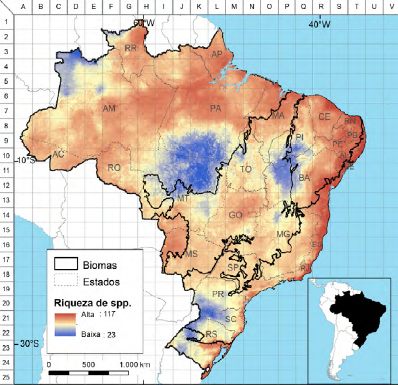
\includegraphics[width=0.8\linewidth]{imagens/figura04} 

}

\caption{Riqueza potencial de espécies de morcegos modelada para o Brasil.}\label{fig:04}
\end{figure}

\begin{figure}

{\centering 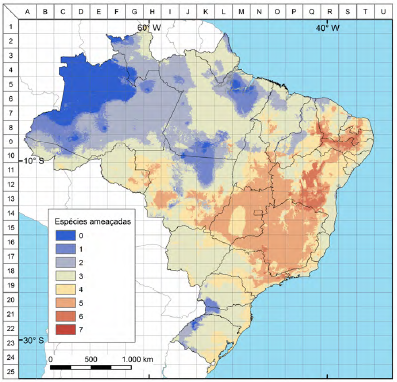
\includegraphics[width=0.8\linewidth]{imagens/figura05} 

}

\caption{Distribuição potencial de espécies ameaçadas de morcegos no Brasil, considerando as sete espécies oficialmente listadas para o país: Eptesicus taddeii (VU), Furipterus horrens (VU), Glyphonycteris behnii (VU), Lonchorhina aurita (VU), Natalus macrourus (VU), Xeronycteris vieirai (VU), e Lonchophylla dekeyseri (EN).}\label{fig:05}
\end{figure}

\hypertarget{cons-finais-morcegos}{%
\section{Considerações finais}\label{cons-finais-morcegos}}

Os dados aqui apresentados apontam claramente uma forte sobreposição entre locais de instalação de parques eólicos e algumas das áreas com maior riqueza potencial e maior potencial de ocorrência de espécies ameaçadas de morcegos no Brasil. Os resultados permitem ainda a identificação de áreas onde esta sobreposição é mais crítica, com a identificação de quadrículas que atualmente contam com mais de 1 milhão de metros quadrados de área de rotor em atividade. É especialmente preocupante que a maior parte destas quadrículas estejam concentradas exatamente em áreas que são grandes vazios amostrais para morcegos no Brasil (Bernard et al.~2011), com ênfase para a Caatinga (Neri et al.~2019). A ausência de informações básicas sobre ocorrência de espécies nestes locais reforça a necessidade de que os Estudos de Impacto Ambiental associados aos parques eólicos sejam bem realizados (veja Bernard et al.~2014; Valença \& Bernard 2015).

\hypertarget{referencias-morcegos}{%
\section{Referências bibliográficas}\label{referencias-morcegos}}

Aguiar, L.M.S.; Bernard, E.; Ribeiro, V.; Machado, R.B. \& Jones, G. 2016. Should I stay or should I go? Climate change effects on the future of Neotropical savannah bats. Global Ecology and Conservation, 5, 22-33.

Arnone, I.S.; Trajano, E.; Pulchério-Leite, A. \& Passos, F.C. 2016. Long-distance movement by a great fruit-eating bat, Artibeus lituratus (Olfers, 1818), in southeastern Brazil (Chiroptera, Phyllostomidae): evidence for migration in Neotropical bats? Biota Neotropica 16(1). \url{http://dx.doi.org/10.1590/1676-0611-BN-2015-0026}

Baerwald, E.F. \& Barclay, R.M.R. 2009. Geographic variation in activity and fatality of migratory bats at wind energy facilities. Journal of Mammalogy 90(6): 1341-1349.

Barros, M.A.S.; Luz, J.L. \& Esberard, C.E.L. 2012. Situação atual da marcação de morcegos no Brasil e perspectivas para a criação de um programa nacional de anilhamento. Chiroptera Neotropical 18:1074-1088.

Barros, M.A.S.; Pessoa, D. \& Rui, A.M. 2014. Habitat use and seasonal activity of insectivorous bats (Mammalia: Chiroptera) in the grasslands of southern Brazil. Zoologia 31(2): 153-161.

Bernard, E.; Paese, A.; Machado, R.B. \& Aguiar, L.M.S. 2014. Blown in the wind: bats and wind farms in Brazil. Natureza \& Conservação 12:106-111.

Bernard, E. \& Saldanha, L.N. 2004. Anilhamento de morcegos: um registro de deslocamento no Pará. In: XXV Congresso Brasileiro de Zoologia, 2004, Brasília, 2004.
Brasil, Conselho Nacional de Meio Ambiente {[}CONAMA{]}. 1997. Resolução nº 237, de 19 de dezembro de 1997. Diário Oficial da União nº 247, de 22 de dezembro de 1997, páginas 30841 a 30843.

Delgado-Jaramillo, M.; Aguiar, L.M.S.; Machado, R.B. \& Bernard, E. Assessing the distribution of a species-rich group in a continental-sized megadiverse country: Bats in Brazil. Diversity \& Distributions. No prelo.

Elith, J.; Graham, C.H;, Anderson, R.P.; Dudı, M.; Ferrier, S.; Guisan, A.; Hijmans, R.J.; Huettmann, F.; Leathwick, J.R.; Lehmann, A.; Li, J.; Lohmann, L.G.; Loiselle, B.A.; Manion, G.; Moritz, C.; Nakamura, M.; Nakazawa, Y.; Overton, J.M.; Peterson, A.T.; Phillips, S.J.; Richardson, K.; Scachetti-pereira, R.; Schapire, R.E.; Williams, S.; Wisz, M.S. \& Zimmermann, N.E. 2006. Novel methods improve prediction of species ' distributions from occurrence data. Ecography 29(2): 129-151.

Esbérard, C.E. 2007. Influência do ciclo lunar na captura de morcegos Phyllostomidae. Iheringia Série Zoologia 97(1): 81-85.

Esbérard, C.E.L.; Godoy, M.S.M.; Renovato, L. \& Carvalho, W.D. 2017. Novel long-distance movements by Neotropical bats (Mammalia: Chiroptera: Phyllostomidae) evidenced by recaptures in southeastern Brazil. Studies on Neotropical Fauna and Environment 52:75-80.

Esbérard, C.E.L.; Godoy, M.S.M.; Renovato, L. \& Carvalho, W.D. 2017. Novel long-distance movements by Neotropical bats (Mammalia: Chiroptera: Phyllostomidae) evidenced by recaptures in southeastern Brazil. Studies on Neotropical Fauna and Environment 52:75-80.

ESRI (Environmental Systems Research Institute). 2013. ArcGIS Professional GIS for the desktop, versão 10.2, 2013.

Farias H.M. 2012. Monitoramento e identificação acústica de espécies de morcegos da Mata Atlântica por sinais de ecolocalização: Contribuições ecológicas e potencial para conservação. Dissertação de Mestrado, Universidade Estadual de Santa Cruz.

Hijmans, R.J.; Cameron, S.E.; Parra, J.L.; Jones, P.G. \& Jarvis, A. 2005. Very high resolution interpolated climate surfaces for global land areas. International Journal of Climatology 25: 1965-1978.

Hintze, F.; Arias-Aguillar, A.; Aguiar, L.M.S.; Pereira, M.J.R. \& Bernard, E. Uma nota de precaução sobre a identificação automática de chamados de ecolocalização de morcegos no Brasil. Boletim da Sociedade Brasileira de Mastozoologia, In press.

Hintze, F.; Duro, V.; Carvalho, J.C.; Eira, C.; Rodrigues, P.C. \& Vingada, J. 2016. Influence of reservoirs created by small dams on the activity of bats. Acta Chiropterologica 18(2): 395-408.

Hull, C.L. \& Muir, S. 2010. Search areas for monitoring bird and bat carcasses at wind farms using a Monte-Carlo model. Australasian Journal of Environmental Management, 17(2): 77-87.

Johnson, G.D.; Erickson, W.P.; Dale Strickland, M.; Shepherd, M.F.; Shepherd, D.A. \& Sarappo, S.A. 2003. Mortality of bats at a large-scale wind power development at Buffalo Ridge, Minnesota. The American Midland Naturalist, 150(2): 332-342.

Kunz, T.H.; Arnett, E.B.; Cooper, B.M.; Erickson, W.P.; Larkin, R.P.; Mabee, T.; Morrison, M.L.; Strickland, M.D.~\& Szewczak, J.M. 2007. Assessing impacts of wind‐energy development on nocturnally active birds and bats: a guidance document. Journal of Wildlife Management, 71(8): 2449-2486.

Kunz, T.H.; Hodgkison, R. \& Weise, C. 2009. Methods of Capturing and Handling Bats, pp.~pp.~3--35. In: T.H. Kunz \& S. Parsons (Eds.). Ecological and behavioral methods for the study of bats. Baltimore, The Johns Hopkins University Press.

López-Baucells, A.; Rocha, R.; Bobrowiec, P.; Bernard, E.; Palmeirim, J. \& Meyer, C. 2016. Field guide to Amazonian bats. Manaus, Editora do INPA. Disponível em: \url{http://tropicalconservation.net/?page_id=10}

Lumsden, L.F. \& Bennett, A.F. 2005. Scattered trees in rural landscapes: foraging habitat for insectivorous bats in southeastern Australia. Biological Conservation 122 (2): 205-222.

Neri, M.; Jameli, D.; Bernard, E. \& Melo, F.P.L. 2019. Green versus green? Adverting potential conflicts between wind power generation and biodiversity conservation in Brazil. Perspectives in Ecology and Conservation. \url{https://doi.org/10.1016/j.pecon.2019.08.004}

Nogueira, M.R.; Lima, I.P.; Garbino, G.S.T.; Moratelli, R.; Tavares, V.C.; Gregorin, R. \& Peracchi, A.L. 2018. Updated checklist of Brazilian bats: version 2018.1. Comitê da Lista de Morcegos do Brasil---CLMB. Sociedade Brasileira para o Estudo de Quirópteros (Sbeq). \url{http://www.sbeq.net/updatelist}

Ontario, Ministry of Natural Resources. 2011. Bats and Bat Habitats: Guidelines for Wind Power Projects, Second Edition. Ontario, Queen's Printer for Ontario. 24p.

Parsons, S. \& Szewczak, J.M. 2009. Detecting, Recording, and Analyzing the Vocalizations of Bats, pp.~91-111. In: T.H. Kunz \& S. Parsons (Eds.). Ecological and behavioral methods for the study of bats. Baltimore, The Johns Hopkins University Press.

Pearson, R.G.; Raxworthy, C.J.; Nakamura, M. \& Townsend Peterson, A. 2006. Predicting species distributions from small numbers of occurrence records: a test case using cryptic geckos in Madagascar. Journal of Biogeography 34, 102-117.

Phillips, S.J.; Anderson, R.P. \& Schapire, R.E. 2006. Maximum entropy modeling of species geographic distributions. Ecological Modelling 190, 231-259.

Red Latinoamericana para la Conservación de los Murciélagos - RELCOM. 2016. Lineamientos de evaluación de impacto ambiental sobre murciélagos por plantas de energía eólica em Latinoamérica y el Caribe. Disponível em: \url{http://www.relcomlatinoamerica.net/images/PDFs/RELCOMEolicasEIA.pdf}

Rodrigues, L.; Bach, L.; Dubourg-Savage, M.-J.; Karapandža, B.; Kovač, D.; Kervyn, T.; Dekker, J.; Kepel, A.; Bach, P.; Collins, J.; Harbusch, C.; Park, K.; Micevski, B. \& Minderman, J. 2015. Guidelines for consideration of bats in wind farm projects ‒ Revision 2014, Eurobats Publication Series No.~6. (English version). Bonn, UNEP/EUROBATS Secretariat. 133p.

Straube, F.C. \& Bianconi, G.V. 2002. Sobre a grandeza e a unidade utilizada para estimar esforço de captura com utilização de redes-de-neblina. Chiroptera Neotropical 8(1-2): 150-152.

Valença, R.B. \& Bernard, E. 2015. Another blown in the wind: bats and the licensing of wind farms in Brazil. Natureza \& Conservação 13:117-122.

Voigt, C.C.; Schneeberger K.; Voigt-Heucke, S.L. \& Lewanzik, D. 2011. Rain increases the energy cost of bat flight. Biology letters, rsbl20110313.

\hypertarget{anexos}{%
\chapter*{Anexos}\label{anexos}}
\addcontentsline{toc}{chapter}{Anexos}

\textbf{Anexo 1.} Espécies de aves migratórias consideradas para a priorização espacial utilizando o Zonation e seus pesos atribuídos (\emph{A = Reprodução exclusiva no Brasil; B = Flocking; C = Voo noturno ou crepuscular; D = Planador; E = Alta sensibilidade aos impactos das estruturas de apoio, exceto colisão; F = Massa corporal média (0,25 qdo \textgreater300g); G = categoria de ameaça; H = PESO FINAL}).

\begin{longtable}{>{}lrrrrrrrr}
\toprule
Espécie & A & B & C & D & E & F & G & H\\
\midrule
\em{Amazona pretrei} & 1 & 1 & 1 & 0 & 1 & 0.25 & 2 & 6.25\\
\em{Calidris canutus} & 0 & 1 & 1 & 0 & 0 & 0.00 & 4 & 6.00\\
\em{Limnodromus griseus} & 0 & 1 & 1 & 0 & 0 & 0.00 & 4 & 6.00\\
\em{Thalasseus maximus} & 0 & 1 & 1 & 0 & 0 & 0.25 & 3 & 5.25\\
\em{Calidris pusilla} & 0 & 1 & 1 & 0 & 0 & 0.00 & 3 & 5.00\\
\addlinespace
\em{Sterna dougallii} & 0 & 1 & 1 & 0 & 1 & 0.00 & 2 & 5.00\\
\em{Tangara peruviana} & 1 & 0 & 1 & 0 & 1 & 0.00 & 2 & 5.00\\
\em{Calidris subruficollis} & 0 & 1 & 1 & 0 & 0 & 0.00 & 2 & 4.00\\
\em{Sporophila beltoni} & 1 & 1 & 0 & 0 & 0 & 0.00 & 2 & 4.00\\
\em{Sporophila melanogaster} & 1 & 1 & 0 & 0 & 0 & 0.00 & 2 & 4.00\\
\addlinespace
\em{Sporophila ruficollis} & 1 & 1 & 0 & 0 & 0 & 0.00 & 2 & 4.00\\
\em{Sterna hirundinacea} & 0 & 1 & 1 & 0 & 0 & 0.00 & 2 & 4.00\\
\em{Coscoroba coscoroba} & 0 & 1 & 1 & 0 & 1 & 0.25 & 0 & 3.25\\
\em{Rostrhamus sociabilis} & 0 & 1 & 1 & 1 & 0 & 0.25 & 0 & 3.25\\
\em{Neochen jubata} & 0 & 1 & 0 & 0 & 1 & 0.25 & 1 & 3.25\\
\addlinespace
\em{Numenius hudsonicus} & 0 & 1 & 1 & 0 & 0 & 0.25 & 1 & 3.25\\
\em{Arenaria interpres} & 0 & 1 & 1 & 0 & 0 & 0.00 & 1 & 3.00\\
\em{Calidris minutilla} & 0 & 1 & 1 & 0 & 0 & 0.00 & 1 & 3.00\\
\em{Casiornis fusca} & 1 & 0 & 1 & 0 & 1 & 0.00 & 0 & 3.00\\
\em{Catharus fuscescens} & 0 & 1 & 1 & 0 & 1 & 0.00 & 0 & 3.00\\
\addlinespace
\em{Catharus minimus} & 0 & 1 & 1 & 0 & 1 & 0.00 & 0 & 3.00\\
\em{Catharus swainsoni} & 0 & 1 & 1 & 0 & 1 & 0.00 & 0 & 3.00\\
\em{Harpagus diodon} & 0 & 1 & 0 & 1 & 1 & 0.00 & 0 & 3.00\\
\em{Phalaropus tricolor} & 0 & 1 & 1 & 0 & 0 & 0.00 & 1 & 3.00\\
\em{Pluvialis dominica} & 0 & 1 & 1 & 0 & 0 & 0.00 & 1 & 3.00\\
\addlinespace
\em{Pygochelidon melanoleuca} & 0 & 1 & 1 & 0 & 0 & 0.00 & 1 & 3.00\\
\em{Sporophila hypoxantha} & 0 & 1 & 0 & 0 & 0 & 0.00 & 2 & 3.00\\
\em{Sporophila palustris} & 0 & 1 & 0 & 0 & 0 & 0.00 & 2 & 3.00\\
\em{Buteo platypterus} & 0 & 1 & 0 & 1 & 0 & 0.25 & 0 & 2.25\\
\em{Buteo swainsoni} & 0 & 1 & 0 & 1 & 0 & 0.25 & 0 & 2.25\\
\addlinespace
\em{Dendrocygna bicolor} & 0 & 1 & 1 & 0 & 0 & 0.25 & 0 & 2.25\\
\em{Elanoides forficatus} & 0 & 1 & 0 & 1 & 0 & 0.25 & 0 & 2.25\\
\em{Larus atlanticus} & 0 & 1 & 1 & 0 & 0 & 0.25 & 0 & 2.25\\
\em{Leucophaeus atricilla} & 0 & 1 & 1 & 0 & 0 & 0.25 & 0 & 2.25\\
\em{Nyctanassa violacea} & 0 & 1 & 1 & 0 & 0 & 0.25 & 0 & 2.25\\
\addlinespace
\em{Phoenicopterus chilensis} & 0 & 1 & 0 & 0 & 1 & 0.25 & 0 & 2.25\\
\em{Platalea ajaja} & 0 & 1 & 0 & 0 & 1 & 0.25 & 0 & 2.25\\
\em{Plegadis chihi} & 0 & 1 & 1 & 0 & 0 & 0.25 & 0 & 2.25\\
\em{Contopus cooperi} & 0 & 0 & 1 & 0 & 0 & 0.00 & 1 & 2.00\\
\em{Sporophila cinnamomea} & 0 & 1 & 0 & 0 & 0 & 0.00 & 1 & 2.00\\
\addlinespace
\em{Actitis macularius} & 0 & 1 & 1 & 0 & 0 & 0.00 & 0 & 2.00\\
\em{Anthracothorax nigricollis} & 0 & 0 & 1 & 0 & 1 & 0.00 & 0 & 2.00\\
\em{Attila phoenicurus} & 0 & 0 & 1 & 0 & 1 & 0.00 & 0 & 2.00\\
\em{Bartramia longicauda} & 0 & 1 & 1 & 0 & 0 & 0.00 & 0 & 2.00\\
\em{Calidris alba} & 0 & 1 & 1 & 0 & 0 & 0.00 & 0 & 2.00\\
\addlinespace
\em{Calidris bairdii} & 0 & 1 & 1 & 0 & 0 & 0.00 & 0 & 2.00\\
\em{Calidris fuscicollis} & 0 & 1 & 1 & 0 & 0 & 0.00 & 0 & 2.00\\
\em{Calidris himantopus} & 0 & 1 & 1 & 0 & 0 & 0.00 & 0 & 2.00\\
\em{Calidris melanotos} & 0 & 1 & 1 & 0 & 0 & 0.00 & 0 & 2.00\\
\em{Charadrius falklandicus} & 0 & 1 & 1 & 0 & 0 & 0.00 & 0 & 2.00\\
\addlinespace
\em{Charadrius modestus} & 0 & 1 & 1 & 0 & 0 & 0.00 & 0 & 2.00\\
\em{Charadrius semipalmatus} & 0 & 1 & 1 & 0 & 0 & 0.00 & 0 & 2.00\\
\em{Chlidonias niger} & 0 & 1 & 1 & 0 & 0 & 0.00 & 0 & 2.00\\
\em{Chordeiles minor} & 0 & 1 & 1 & 0 & 0 & 0.00 & 0 & 2.00\\
\em{Coccyzus americanus} & 0 & 0 & 1 & 0 & 1 & 0.00 & 0 & 2.00\\
\addlinespace
\em{Coccyzus melacoryphus} & 0 & 0 & 1 & 0 & 1 & 0.00 & 0 & 2.00\\
\em{Dacnis nigripes} & 1 & 0 & 0 & 0 & 1 & 0.00 & 0 & 2.00\\
\em{Florisuga fusca} & 0 & 0 & 1 & 0 & 1 & 0.00 & 0 & 2.00\\
\em{Gelochelidon nilotica} & 0 & 1 & 1 & 0 & 0 & 0.00 & 0 & 2.00\\
\em{Hirundo rustica} & 0 & 1 & 1 & 0 & 0 & 0.00 & 0 & 2.00\\
\addlinespace
\em{Ictinia mississippiensis} & 0 & 1 & 0 & 1 & 0 & 0.00 & 0 & 2.00\\
\em{Ictinia plumbea} & 0 & 1 & 0 & 1 & 0 & 0.00 & 0 & 2.00\\
\em{Inezia inornata} & 0 & 0 & 1 & 0 & 1 & 0.00 & 0 & 2.00\\
\em{Lessonia rufa} & 0 & 0 & 1 & 0 & 1 & 0.00 & 0 & 2.00\\
\em{Limosa haemastica} & 0 & 1 & 1 & 0 & 0 & 0.00 & 0 & 2.00\\
\addlinespace
\em{Myiophobus fasciatus} & 0 & 1 & 1 & 0 & 0 & 0.00 & 0 & 2.00\\
\em{Oreopholus ruficollis} & 0 & 1 & 1 & 0 & 0 & 0.00 & 0 & 2.00\\
\em{Pardirallus sanguinolentus} & 0 & 1 & 1 & 0 & 0 & 0.00 & 0 & 2.00\\
\em{Petrochelidon pyrrhonota} & 0 & 1 & 1 & 0 & 0 & 0.00 & 0 & 2.00\\
\em{Piranga rubra} & 0 & 0 & 1 & 0 & 1 & 0.00 & 0 & 2.00\\
\addlinespace
\em{Pitangus sulphuratus} & 0 & 1 & 1 & 0 & 0 & 0.00 & 0 & 2.00\\
\em{Pluvialis squatarola} & 0 & 1 & 1 & 0 & 0 & 0.00 & 0 & 2.00\\
\em{Podager nacunda} & 0 & 1 & 1 & 0 & 0 & 0.00 & 0 & 2.00\\
\em{Progne chalybea} & 0 & 1 & 1 & 0 & 0 & 0.00 & 0 & 2.00\\
\em{Progne elegans} & 0 & 1 & 1 & 0 & 0 & 0.00 & 0 & 2.00\\
\addlinespace
\em{Progne subis} & 0 & 1 & 1 & 0 & 0 & 0.00 & 0 & 2.00\\
\em{Progne tapera} & 0 & 1 & 1 & 0 & 0 & 0.00 & 0 & 2.00\\
\em{Pseudocolopteryx acutipennis} & 0 & 0 & 1 & 0 & 1 & 0.00 & 0 & 2.00\\
\em{Riparia riparia} & 0 & 1 & 1 & 0 & 0 & 0.00 & 0 & 2.00\\
\em{Rynchops niger} & 0 & 1 & 1 & 0 & 0 & 0.00 & 0 & 2.00\\
\addlinespace
\em{Stelgidopteryx ruficollis} & 0 & 1 & 1 & 0 & 0 & 0.00 & 0 & 2.00\\
\em{Sterna hirundo} & 0 & 1 & 1 & 0 & 0 & 0.00 & 0 & 2.00\\
\em{Sterna paradisaea} & 0 & 1 & 1 & 0 & 0 & 0.00 & 0 & 2.00\\
\em{Sterna trudeaui} & 0 & 1 & 1 & 0 & 0 & 0.00 & 0 & 2.00\\
\em{Sternula antillarum} & 0 & 1 & 1 & 0 & 0 & 0.00 & 0 & 2.00\\
\addlinespace
\em{Tachycineta leucopyga} & 0 & 1 & 1 & 0 & 0 & 0.00 & 0 & 2.00\\
\em{Tersina viridis} & 0 & 1 & 1 & 0 & 0 & 0.00 & 0 & 2.00\\
\em{Thalasseus acuflavidus} & 0 & 1 & 1 & 0 & 0 & 0.00 & 0 & 2.00\\
\em{Tringa flavipes} & 0 & 1 & 1 & 0 & 0 & 0.00 & 0 & 2.00\\
\em{Tringa melanoleuca} & 0 & 1 & 1 & 0 & 0 & 0.00 & 0 & 2.00\\
\addlinespace
\em{Tringa semipalmata} & 0 & 1 & 1 & 0 & 0 & 0.00 & 0 & 2.00\\
\em{Turdus flavipes} & 0 & 1 & 1 & 0 & 0 & 0.00 & 0 & 2.00\\
\em{Tyrannus savana} & 0 & 1 & 1 & 0 & 0 & 0.00 & 0 & 2.00\\
\em{Tyrannus tyrannus} & 0 & 1 & 1 & 0 & 0 & 0.00 & 0 & 2.00\\
\em{Vireo altiloquus} & 0 & 0 & 1 & 0 & 1 & 0.00 & 0 & 2.00\\
\addlinespace
\em{Vireo chivi} & 0 & 0 & 1 & 0 & 1 & 0.00 & 0 & 2.00\\
\em{Vireo olivaceus} & 0 & 0 & 1 & 0 & 1 & 0.00 & 0 & 2.00\\
\em{Anas discors} & 0 & 1 & 0 & 0 & 0 & 0.25 & 0 & 1.25\\
\em{Anas georgica} & 0 & 1 & 0 & 0 & 0 & 0.25 & 0 & 1.25\\
\em{Anas platalea} & 0 & 1 & 0 & 0 & 0 & 0.25 & 0 & 1.25\\
\addlinespace
\em{Anas sibilatrix} & 0 & 1 & 0 & 0 & 0 & 0.25 & 0 & 1.25\\
\em{Anas versicolor} & 0 & 1 & 0 & 0 & 0 & 0.25 & 0 & 1.25\\
\em{Callonetta leucophrys} & 0 & 1 & 0 & 0 & 0 & 0.25 & 0 & 1.25\\
\em{Falco peregrinus} & 0 & 0 & 0 & 1 & 0 & 0.25 & 0 & 1.25\\
\em{Heteronetta atricapilla} & 0 & 1 & 0 & 0 & 0 & 0.25 & 0 & 1.25\\
\addlinespace
\em{Netta peposaca} & 0 & 1 & 0 & 0 & 0 & 0.25 & 0 & 1.25\\
\em{Oxyura vittata} & 0 & 1 & 0 & 0 & 0 & 0.25 & 0 & 1.25\\
\em{Pandion haliaetus} & 0 & 0 & 0 & 1 & 0 & 0.25 & 0 & 1.25\\
\em{Chaetura meridionalis} & 0 & 1 & 0 & 0 & 0 & 0.00 & 0 & 1.00\\
\em{Cinclodes fuscus} & 0 & 1 & 0 & 0 & 0 & 0.00 & 0 & 1.00\\
\addlinespace
\em{Contopus virens} & 0 & 0 & 1 & 0 & 0 & 0.00 & 0 & 1.00\\
\em{Cyanoloxia glaucocaerulea} & 0 & 0 & 0 & 0 & 1 & 0.00 & 0 & 1.00\\
\em{Dolichonyx oryzivorus} & 0 & 1 & 0 & 0 & 0 & 0.00 & 0 & 1.00\\
\em{Elaenia chilensis} & 0 & 0 & 1 & 0 & 0 & 0.00 & 0 & 1.00\\
\em{Elaenia chiriquensis} & 0 & 0 & 1 & 0 & 0 & 0.00 & 0 & 1.00\\
\addlinespace
\em{Elaenia parvirostris} & 0 & 0 & 1 & 0 & 0 & 0.00 & 0 & 1.00\\
\em{Elaenia spectabilis} & 0 & 0 & 1 & 0 & 0 & 0.00 & 0 & 1.00\\
\em{Empidonax alnorum} & 0 & 0 & 1 & 0 & 0 & 0.00 & 0 & 1.00\\
\em{Empidonomus varius} & 0 & 0 & 1 & 0 & 0 & 0.00 & 0 & 1.00\\
\em{Fluvicola albiventer} & 0 & 0 & 1 & 0 & 0 & 0.00 & 0 & 1.00\\
\addlinespace
\em{Griseotyrannus aurantioatrocristatus} & 0 & 0 & 1 & 0 & 0 & 0.00 & 0 & 1.00\\
\em{Hydropsalis parvulus} & 0 & 0 & 1 & 0 & 0 & 0.00 & 0 & 1.00\\
\em{Hymenops perspicillatus} & 0 & 0 & 1 & 0 & 0 & 0.00 & 0 & 1.00\\
\em{Lathrotriccus euleri} & 0 & 0 & 1 & 0 & 0 & 0.00 & 0 & 1.00\\
\em{Legatus leucophaius} & 0 & 0 & 1 & 0 & 0 & 0.00 & 0 & 1.00\\
\addlinespace
\em{Lurocalis semitorquatus} & 0 & 0 & 1 & 0 & 0 & 0.00 & 0 & 1.00\\
\em{Micrococcyx cinereus} & 0 & 0 & 1 & 0 & 0 & 0.00 & 0 & 1.00\\
\em{Myiarchus swainsoni} & 0 & 0 & 1 & 0 & 0 & 0.00 & 0 & 1.00\\
\em{Myiodynastes maculatus} & 0 & 0 & 1 & 0 & 0 & 0.00 & 0 & 1.00\\
\em{Myiopagis viridicata} & 0 & 0 & 1 & 0 & 0 & 0.00 & 0 & 1.00\\
\addlinespace
\em{Pachyramphus polychopterus} & 0 & 0 & 1 & 0 & 0 & 0.00 & 0 & 1.00\\
\em{Pachyramphus validus} & 0 & 0 & 1 & 0 & 0 & 0.00 & 0 & 1.00\\
\em{Porphyrio martinicus} & 0 & 0 & 1 & 0 & 0 & 0.00 & 0 & 1.00\\
\em{Pseudocolopteryx flaviventris} & 0 & 0 & 1 & 0 & 0 & 0.00 & 0 & 1.00\\
\em{Pyrocephalus rubinus} & 0 & 0 & 1 & 0 & 0 & 0.00 & 0 & 1.00\\
\addlinespace
\em{Serpophaga griseicapilla} & 0 & 0 & 1 & 0 & 0 & 0.00 & 0 & 1.00\\
\em{Serpophaga munda} & 0 & 0 & 1 & 0 & 0 & 0.00 & 0 & 1.00\\
\em{Setophaga petechia} & 0 & 0 & 1 & 0 & 0 & 0.00 & 0 & 1.00\\
\em{Setophaga ruticilla} & 0 & 0 & 1 & 0 & 0 & 0.00 & 0 & 1.00\\
\em{Setophaga striata} & 0 & 0 & 1 & 0 & 0 & 0.00 & 0 & 1.00\\
\addlinespace
\em{Sporophila bouvreuil} & 0 & 1 & 0 & 0 & 0 & 0.00 & 0 & 1.00\\
\em{Sporophila caerulescens} & 0 & 1 & 0 & 0 & 0 & 0.00 & 0 & 1.00\\
\em{Sporophila hypochroma} & 0 & 1 & 0 & 0 & 0 & 0.00 & 0 & 1.00\\
\em{Sporophila lineola} & 0 & 1 & 0 & 0 & 0 & 0.00 & 0 & 1.00\\
\em{Sublegatus modestus} & 0 & 0 & 1 & 0 & 0 & 0.00 & 0 & 1.00\\
\addlinespace
\em{Tringa solitaria} & 0 & 0 & 1 & 0 & 0 & 0.00 & 0 & 1.00\\
\em{Turdus amaurochalinus} & 0 & 0 & 1 & 0 & 0 & 0.00 & 0 & 1.00\\
\em{Turdus subalaris} & 0 & 0 & 1 & 0 & 0 & 0.00 & 0 & 1.00\\
\em{Tyrannus albogularis} & 0 & 0 & 1 & 0 & 0 & 0.00 & 0 & 1.00\\
\em{Tyrannus melancholicus} & 0 & 0 & 1 & 0 & 0 & 0.00 & 0 & 1.00\\
\addlinespace
\em{Xolmis coronata} & 0 & 0 & 1 & 0 & 0 & 0.00 & 0 & 1.00\\
\em{Chionis albus} & 0 & 0 & 0 & 0 & 0 & 0.25 & 0 & 0.25\\
\em{Anthus correndera} & 0 & 0 & 0 & 0 & 0 & 0.00 & 0 & 0.00\\
\em{Mimus triurus} & 0 & 0 & 0 & 0 & 0 & 0.00 & 0 & 0.00\\
\em{Pheucticus aureoventris} & 0 & 0 & 0 & 0 & 0 & 0.00 & 0 & 0.00\\
\addlinespace
\em{Phytotoma rutila} & 0 & 0 & 0 & 0 & 0 & 0.00 & 0 & 0.00\\
\bottomrule
\end{longtable}

\textbf{Anexo 2.} Parâmetros definidos para execução da priorização no Zonation.

{[}Settings{]}\\
removal rule = 2\\
edge removal = 1\\
add edge points = 1\\
warp factor = 1\\
use mask = 0\\
use planning unit layer = 0\\
use groups = 0\\
use condition layer = 0\\
mask missing areas = 0\\
{[}Transformed layers{]}\\
output condition transformed

  \bibliography{book.bib,packages.bib}

\end{document}
